\documentclass[preview]{standalone}

\usepackage[utf8]{inputenc}
\usepackage{amsmath, amssymb}
\usepackage{graphicx}
\usepackage{subcaption}

% Matplotlib2TikZ
\usepackage{pgfplots}
\pgfplotsset{compat=1.14}

\begin{document}
\begin{minipage}{19.05cm}
\begin{figure}
	\centering
	\begin{subfigure}[t]{8.8cm}
	    \centering
	    % This file was created by matplotlib2tikz v0.6.11.
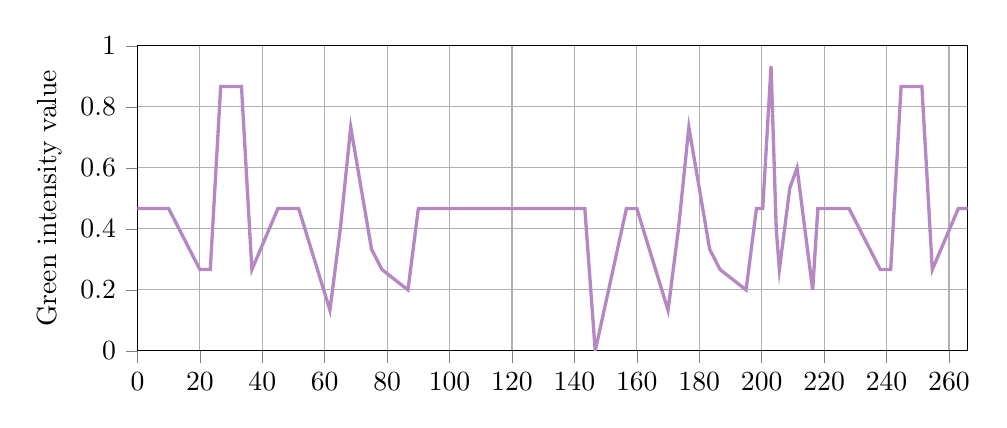
\begin{tikzpicture}

\definecolor{color0}{rgb}{0.7109375,0.53515625,0.76953125}

\begin{axis}[
width=\textwidth,
height=0.45\textwidth,
% xlabel={Time [s]},
ylabel={Green intensity value},
xmin=0, xmax=266,
ymin=0, ymax=1,
tick align=outside,
tick pos=left,
xmajorgrids,
ymajorgrids,
x grid style={lightgray!92.026143790849673!black},
y grid style={lightgray!92.026143790849673!black}
]
\addplot [very thick, color0, forget plot]
table {%
0 0.4666666667
10 0.4666666667
20 0.2666666667
23.3333333333 0.2666666667
26.6666666667 0.8666666667
33.3333333333 0.8666666667
36.6666666667 0.2666666667
45 0.4666666667
48.3333333333 0.4666666667
51.6666666667 0.4666666667
61.6666666667 0.1333333333
65 0.4
68.3333333333 0.7333333333
75 0.3333333333
78.3333333333 0.2666666667
86.6666666667 0.2
90 0.4666666667
143.3333333333 0.4666666667
146.6666666667 0
156.6666666667 0.4666666667
160 0.4666666667
170 0.1333333333
173.3333333333 0.4
176.6666666667 0.7333333333
183.3333333333 0.3333333333
186.6666666666 0.2666666667
195 0.2
198.3333333333 0.4666666667
200.3333333333 0.4666666667
203 0.9333333333
204.6666666666 0.4
205.6666666666 0.2666666667
209 0.5333333333
211.3333333333 0.6
216.3333333333 0.2
218 0.4666666667
228 0.4666666667
238 0.2666666667
241.3333333333 0.2666666667
244.6666666666 0.8666666667
251.3333333333 0.8666666667
254.6666666666 0.2666666667
263 0.4666666667
266.3333333333 0.4666666667
};
\end{axis}

\end{tikzpicture}\label{Fig2a}
	    \caption{Task A: Ground truth}
    \end{subfigure}
	~
	\begin{subfigure}[t]{8.8cm}
    	\centering
    	% This file was created by matplotlib2tikz v0.6.11.
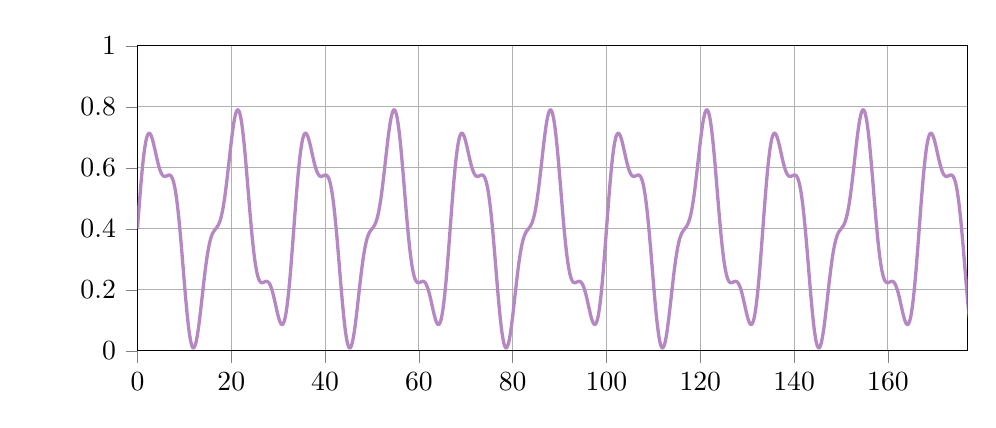
\begin{tikzpicture}

\definecolor{color0}{rgb}{0.7109375,0.53515625,0.76953125}

\begin{axis}[
width=\textwidth,
height=0.45\textwidth,
% xlabel={Time [s]},
%ylabel={Green intensity value},
ylabel={\phantom{Green intensity value}},
xmin=0, xmax=177,
ymin=0, ymax=1,
tick align=outside,
tick pos=left,
xmajorgrids,
ymajorgrids,
x grid style={lightgray!92.026143790849673!black},
y grid style={lightgray!92.026143790849673!black}
]
\addplot [very thick, color0, forget plot]
table {%
0 0.4
0.1 0.420715117915489
0.2 0.4413306579254
0.3 0.461747806202643
0.4 0.481869270465313
0.5 0.501600024278232
0.6 0.520848031752353
0.7 0.539524946378326
0.8 0.557546777959114
0.9 0.574834521888531
1 0.591314745355334
1.1 0.60692012543318
1.2 0.621589934441882
1.3 0.635270468431336
1.4 0.647915415141923
1.5 0.659486158329853
1.6 0.669952015907932
1.7 0.679290409936652
1.8 0.687486967102211
1.9 0.694535548931591
2 0.700438211614877
2.1 0.705205095925955
2.2 0.708854248349147
2.3 0.711411375125761
2.4 0.712909531525551
2.5 0.713388749218427
2.6 0.712895605166515
2.7 0.711482735970772
2.8 0.709208302085515
2.9 0.706135406753981
3 0.702331474914616
3.1 0.697867597677625
3.2 0.692817848271335
3.3 0.687258575605452
3.4 0.681267681791179
3.5 0.674923890094628
3.6 0.668306009878904
3.7 0.661492205110867
3.8 0.654559272970815
3.9 0.647581939007397
4 0.640632175126987
4.1 0.633778546497708
4.2 0.627085593185324
4.3 0.620613252023514
4.4 0.614416323857556
4.5 0.608543990891256
4.6 0.603039388415846
4.7 0.597939234710461
4.8 0.59327352238106
4.9 0.589065273852989
5 0.585330363156591
5.1 0.582077405550569
5.2 0.579307715919446
5.3 0.577015336264828
5.4 0.575187131990816
5.5 0.57380295606725
5.6 0.572835879546049
5.7 0.572252486311105
5.8 0.572013229366335
5.9 0.57207284541462
5.99999999999999 0.572380823957502
6.09999999999999 0.572881926656162
6.19999999999999 0.573516752242877
6.29999999999999 0.574222341862731
6.39999999999999 0.574932819361549
6.49999999999999 0.575580060721052
6.59999999999999 0.576094386578898
6.69999999999999 0.576405271561922
6.79999999999999 0.576442064007363
6.89999999999999 0.576134709550597
6.99999999999999 0.57541447201964
7.09999999999999 0.574214645096919
7.19999999999999 0.572471248287232
7.29999999999999 0.570123700866805
7.39999999999999 0.567115467680746
7.49999999999999 0.563394670903141
7.59999999999999 0.558914662173533
7.69999999999999 0.553634549872779
7.79999999999999 0.547519676697246
7.89999999999999 0.540542043129491
7.99999999999999 0.532680672882042
8.09999999999999 0.523921916904418
8.19999999999999 0.514259693087589
8.29999999999998 0.503695659369747
8.39999999999999 0.492239318537638
8.49999999999999 0.479908053623362
8.59999999999999 0.466727093412326
8.69999999999999 0.452729408198222
8.79999999999998 0.437955536540274
8.89999999999998 0.422453344390753
8.99999999999998 0.406277718561755
9.09999999999998 0.389490197083881
9.19999999999998 0.372158539570765
9.29999999999998 0.354356241237252
9.39999999999998 0.336161994720774
9.49999999999998 0.317659104320572
9.59999999999998 0.298934857693862
9.69999999999998 0.280079860427904
9.79999999999998 0.261187339238976
9.89999999999998 0.242352419830463
9.99999999999998 0.223671385670147
10.1 0.205240924119288
10.2 0.187157366461756
10.3 0.169515928439171
10.4 0.152409957897282
10.5 0.135930196089687
10.6 0.120164059067902
10.7 0.10519494541284
10.8 0.0911015763334721
10.9 0.0779573738758097
11 0.065829882651933
11.1 0.0547802401174936
11.2 0.0448627000003429
11.3 0.0361242130164528
11.4 0.0286040685062246
11.5 0.0223336000890968
11.6 0.0173359578717907
11.7 0.0136259491605709
11.8 0.0112099490257261
11.9 0.0100858814524281
12 0.0102432711916508
12.1 0.0116633658034179
12.2 0.014319326767814
12.3 0.0181764879323968
12.4 0.0231926789732688
12.5 0.0293186109763468
12.6 0.0364983207003615
12.7 0.0446696695686551
12.8 0.0537648929574801
12.9 0.0637111949084896
13 0.0744313829963256
13.1 0.0858445377322048
13.2 0.0978667105842194
13.3 0.110411644447422
13.4 0.123391510203803
13.5 0.136717652875692
13.6 0.150301340797182
13.7 0.164054511207501
13.8 0.177890505708061
13.9 0.19172478912087
14 0.205475645439184
14.1 0.219064844770376
14.2 0.232418275434153
14.3 0.245466535694066
14.4 0.258145479963973
14.5 0.270396714740495
14.6 0.282168039963882
14.7 0.293413831999066
14.8 0.304095364951739
14.9 0.314181067586273
15 0.32364671368843
15.1 0.332475544310916
15.2 0.340658320948548
15.3 0.348193309306886
15.4 0.355086193947991
15.5 0.361349924714087
15.6 0.367004496438822
15.7 0.372076664051125
15.8 0.376599595753069
15.9 0.380612467505543
16 0.384160002579001
16.1 0.387291960416443
16.2 0.390062579507774
16.3 0.392529979384679
16.4 0.394755527209638
16.5 0.396803174748287
16.6 0.398738771778384
16.7 0.400629362198614
16.8 0.402542469254725
16.9 0.404545376397456
17 0.406704410325644
17.1 0.409084232748452
17.2 0.41174714732291
17.3 0.414752428087733
17.4 0.418155675522739
17.5 0.42200820611698
17.6 0.426356481029952
17.7 0.431241579081758
17.8 0.436698718912896
17.9 0.44275683471588
18 0.449438209463242
18.1 0.456758169043634
18.2 0.464724840174499
18.3 0.473338974390788
18.4 0.482593839819645
18.5 0.492475181845978
18.6 0.502961253158862
18.7 0.514022913049189
18.8 0.525623795210378
18.9 0.537720542681854
19 0.55026310797475
19.1 0.563195115836284
19.2 0.576454285548641
19.3 0.589972909124981
19.4 0.6036783812641
19.5 0.617493776460769
19.6 0.631338468244948
19.7 0.645128785143813
19.8 0.658778697629023
19.9 0.672200530031026
20 0.685305691174878
20.1 0.698005417319979
20.2 0.710211520871048
20.3 0.721837138270361
20.4 0.732797470482451
20.5 0.743010509542069
20.6 0.752397744753633
20.7 0.760884842304746
20.8 0.76840229228601
20.9 0.774886017392279
21 0.780277937914242
21.1 0.784526488010778
21.2 0.787587078678537
21.3 0.789422503301919
21.4 0.790003282169865
21.5 0.789307942881227
21.6 0.787323234123194
21.7 0.784044270892306
21.8 0.779474609829829
21.9 0.773626253957403
22 0.766519586719291
22.1 0.758183235859052
22.2 0.74865386827518
22.3 0.737975917607029
22.4 0.726201246893605
22.5000000000001 0.713388749218423
22.6000000000001 0.699603889798454
22.7000000000001 0.684918193489499
22.8000000000001 0.669408682159475
22.9000000000001 0.653157266820878
23.0000000000001 0.636250099810196
23.1000000000001 0.618776892651807
23.2000000000001 0.600830205543711
23.3000000000001 0.582504714649793
23.4000000000001 0.56389646357591
23.5000000000001 0.545102105543249
23.6000000000001 0.526218142850956
23.7000000000001 0.507340170240279
23.8000000000001 0.488562128734155
23.9000000000001 0.469975576429794
24.0000000000001 0.451668982568073
24.1000000000001 0.433727050993955
24.2000000000001 0.416230078858423
24.3000000000001 0.399253356097089
24.4000000000001 0.382866610856272
24.5000000000001 0.367133505627414
24.6000000000001 0.352111188398704
24.7000000000001 0.337849902642739
24.8000000000001 0.324392659435408
24.9000000000001 0.311774974448496
25.0000000000001 0.300024671981709
25.1000000000001 0.28916175760405
25.2000000000001 0.27919836036502
25.3000000000001 0.270138744918368
25.4000000000001 0.261979393280551
25.5000000000001 0.254709155328246
25.6000000000001 0.248309466529593
25.7000000000001 0.242754630807797
25.8000000000001 0.238012165858578
25.9000000000001 0.234043207689804
26.0000000000001 0.230802970627417
26.1000000000001 0.228241258541127
26.2000000000001 0.226303022590615
26.3000000000001 0.224928960382204
26.4000000000001 0.224056151060764
26.5000000000001 0.223618720545221
26.6000000000001 0.223548530851321
26.7000000000001 0.223775887234481
26.8000000000001 0.224230256730652
26.9000000000001 0.224840991575371
27.0000000000001 0.22553805094152
27.1000000000001 0.226252714455083
27.2000000000001 0.226918281025188
27.3000000000001 0.227470746659284
27.4000000000001 0.227849455125243
27.5000000000001 0.227997715567733
27.6000000000001 0.227863381484278
27.7000000000001 0.227399385814273
27.8000000000001 0.226564227288819
27.9000000000001 0.225322403627057
28.0000000000001 0.22364478764178
28.1000000000001 0.221508942829335
28.2000000000001 0.218899375561526
28.3000000000001 0.215807721565678
28.4000000000001 0.21223286496807
28.5000000000001 0.208180988780442
28.6000000000001 0.20366555632378
28.7000000000001 0.19870722370267
28.8000000000001 0.193333684061679
28.9000000000001 0.187579444966907
29.0000000000001 0.181485540855761
29.1000000000001 0.175099183080623
29.2000000000001 0.168473350632365
29.3000000000001 0.161666325162606
29.4000000000001 0.154741174424388
29.5000000000001 0.147765188715221
29.6000000000001 0.140809275330017
29.7000000000001 0.133947316410548
29.8000000000002 0.127255495909359
29.9000000000002 0.12081160166655
30.0000000000002 0.114694308825118
30.1000000000002 0.108982450982438
30.2000000000002 0.103754285590563
30.3000000000002 0.0990867601752705
30.4000000000002 0.0950547859425784
30.5000000000002 0.0917305252819351
30.6000000000002 0.0891826995578737
30.7000000000002 0.0874759234076627
30.8000000000002 0.0866700715329796
30.9000000000002 0.0868196836908103
31.0000000000002 0.087973413255244
31.1000000000002 0.0901735243404601
31.2000000000002 0.0934554420494055
31.3000000000002 0.097847359946222
31.4000000000002 0.103369908347495
31.5000000000002 0.110035886492356
31.6000000000002 0.117850061089094
31.7000000000002 0.126809033151233
31.8000000000002 0.136901174434151
31.9000000000002 0.148106634169635
32.0000000000002 0.160397416175695
32.1000000000002 0.17373752579802
32.2000000000002 0.188083185523115
32.3000000000002 0.203383117496951
32.4000000000002 0.219578890592177
32.5000000000002 0.236605329096876
32.6000000000002 0.254390979553577
32.7000000000002 0.272858631763498
32.8000000000002 0.29192588949244
32.9000000000002 0.311505785975602
33.0000000000002 0.331507438922655
33.1000000000002 0.351836739375381
33.2000000000002 0.372397068470928
33.3000000000002 0.393090035917128
33.4000000000002 0.4138162337944
33.5000000000002 0.434475999163258
33.6000000000002 0.454970178878656
33.7000000000002 0.475200889992851
33.8000000000002 0.495072269167469
33.9000000000002 0.514491204612649
34.0000000000002 0.533368044225521
34.1000000000002 0.551617273810709
34.2000000000002 0.56915815952994
34.3000000000002 0.585915349043997
34.4000000000002 0.60181942617532
34.5000000000002 0.616807414330258
34.6000000000002 0.630823224372758
34.7000000000002 0.64381804313201
34.8000000000002 0.655750659251026
34.9000000000002 0.666587723636539
35.0000000000002 0.676303942348152
35.1000000000002 0.68488220036118
35.2000000000002 0.692313615247829
35.3000000000002 0.698597520439822
35.4000000000002 0.703741378356857
35.5000000000002 0.707760624303837
35.6000000000002 0.710678442650154
35.7000000000002 0.712525477401039
35.8000000000002 0.713339479848836
35.9000000000002 0.713164896545855
36.0000000000002 0.712052401365314
36.1000000000002 0.710058375908197
36.2000000000002 0.707244342967156
36.3000000000002 0.703676358170002
36.4000000000002 0.699424365291084
36.5000000000002 0.694561521035824
36.6000000000003 0.689163495368951
36.7000000000002 0.683307753668289
36.8000000000002 0.677072827141403
36.9000000000003 0.670537578040602
37.0000000000003 0.663780466251943
37.1000000000003 0.656878823815535
37.2000000000003 0.649908143857842
37.3000000000003 0.642941390282548
37.4000000000003 0.636048334375928
37.5000000000003 0.629294924237484
37.6000000000003 0.622742692648836
37.7000000000003 0.61644820864629
37.8000000000003 0.610462577668176
37.9000000000003 0.604830994710463
38.0000000000003 0.599592354447269
38.1000000000003 0.594778921760825
38.2000000000003 0.59041606558291
38.3000000000003 0.586522058381438
38.4000000000003 0.583107943036938
38.5000000000003 0.580177468249228
38.6000000000003 0.577727093000126
38.7000000000003 0.575746059978953
38.8000000000003 0.574216537259437
38.9000000000003 0.573113826904818
39.0000000000003 0.57240663857806
39.1000000000003 0.572057425651285
39.2000000000003 0.572022780748151
39.3000000000003 0.572253887119807
39.4000000000003 0.572697021754076
39.5000000000003 0.573294105653022
39.6000000000003 0.573983296290249
39.7000000000003 0.574699616879919
39.8000000000003 0.575375616757835
39.9000000000003 0.575942056894183
40.0000000000003 0.576328614329855
40.1000000000003 0.576464599156072
40.2000000000003 0.576279677541437
40.3000000000003 0.57570459425301
40.4000000000003 0.574671888118609
40.5000000000003 0.573116593936722
40.6000000000003 0.570976924457249
40.7000000000003 0.5681949262301
40.8000000000003 0.56471710334761
40.9000000000003 0.56049500338902
41.0000000000003 0.555485760208245
41.1000000000003 0.549652588586927
41.2000000000003 0.542965226199936
41.3000000000003 0.535400318806359
41.4000000000003 0.526941745081309
41.5000000000003 0.517580878038295
41.6000000000003 0.507316780553615
41.7000000000003 0.496156333088222
41.8000000000003 0.484114292303751
41.9000000000003 0.471213279882301
42.0000000000003 0.45748370147901
42.1000000000003 0.442963596356596
42.2000000000003 0.427698418866731
42.3000000000003 0.411740753548499
42.4000000000003 0.395149966204326
42.5000000000003 0.37799179388299
42.6000000000003 0.360337877242926
42.7000000000003 0.342265239281951
42.8000000000003 0.323855714897405
42.9000000000003 0.305195336179015
43.0000000000003 0.28637367873205
43.1000000000003 0.267483174676555
43.2000000000003 0.248618398266973
43.3000000000003 0.229875330322326
43.4000000000003 0.211350607848308
43.5000000000003 0.193140765367393
43.6000000000003 0.175341474550147
43.7000000000004 0.158046788759729
43.8000000000004 0.141348399081872
43.9000000000004 0.125334908314738
44.0000000000004 0.110091129237969
44.1000000000004 0.0956974132691215
44.2000000000004 0.0822290153506507
44.3000000000004 0.0697555005937677
44.4000000000004 0.0583401978398049
44.5000000000004 0.048039704888402
44.6000000000004 0.0389034496884338
44.7000000000004 0.0309733112962757
44.8000000000004 0.0242833038809799
44.9000000000004 0.0188593265019769
45.0000000000004 0.0147189808068302
45.1000000000004 0.011871458199562
45.2000000000004 0.0103174974193753
45.3000000000004 0.0100494128506559
45.4000000000004 0.0110511932634212
45.5000000000004 0.013298670064419
45.6000000000004 0.0167597535283248
45.7000000000004 0.02139473488139
45.8000000000004 0.0271566515316962
45.9000000000004 0.0339917121860715
46.0000000000004 0.0418397780685264
46.1000000000004 0.0506348959635477
46.2000000000004 0.0603058783539807
46.3000000000004 0.0707769255116431
46.4000000000004 0.0819682840328441
46.5000000000004 0.0937969359938707
46.6000000000004 0.106177312636081
46.7000000000004 0.119022026278852
46.8000000000004 0.132242614003059
46.9000000000004 0.145750286549585
47.0000000000004 0.159456675837132
47.1000000000004 0.173274574522012
47.2000000000004 0.187118661099179
47.3000000000004 0.200906204178042
47.4000000000004 0.214557739757213
47.5000000000004 0.22799771556776
47.6000000000004 0.241155096852362
47.7000000000004 0.253963928295569
47.8000000000004 0.266363847214879
47.9000000000004 0.27830054356018
48.0000000000004 0.289726162746219
48.1000000000004 0.300599647855171
48.2000000000004 0.310887018289167
48.3000000000004 0.320561582521354
48.4000000000004 0.329604083183354
48.5000000000004 0.338002773331836
48.6000000000004 0.34575342335174
48.7000000000004 0.35285925857327
48.8000000000004 0.35933082829835
48.9000000000004 0.36518580754452
49.0000000000004 0.370448733414683
49.1000000000004 0.375150678584385
49.2000000000004 0.379328864959274
49.3000000000004 0.383026221089037
49.4000000000004 0.386290887425678
49.5000000000004 0.389175673979068
49.6000000000004 0.391737475347163
49.7000000000004 0.394036648478275
49.8000000000004 0.396136358855016
49.9000000000004 0.398101901071047
50.0000000000004 0.400000000000004
50.1000000000004 0.401898098928961
50.2000000000004 0.403863641144993
50.3000000000005 0.405963351521734
50.4000000000005 0.408262524652848
50.5000000000005 0.410824326020943
50.6000000000005 0.413709112574335
50.7000000000005 0.416973778910978
50.8000000000005 0.420671135040744
50.9000000000005 0.424849321415634
51.0000000000005 0.429551266585338
51.1000000000005 0.434814192455504
51.2000000000005 0.440669171701677
51.3000000000005 0.44714074142676
51.4000000000005 0.454246576648292
51.5000000000005 0.461997226668199
51.6000000000005 0.470395916816684
51.7000000000005 0.479438417478687
51.8000000000005 0.489112981710875
51.9000000000005 0.499400352144875
52.0000000000005 0.510273837253829
52.1000000000005 0.521699456439871
52.2000000000005 0.533636152785173
52.3000000000005 0.546036071704487
52.4000000000005 0.558844903147694
52.5000000000005 0.572002284432298
52.6000000000005 0.585442260242846
52.7000000000005 0.599093795822018
52.8000000000005 0.61288133890088
52.9000000000005 0.626725425478048
53.0000000000005 0.640543324162928
53.1000000000005 0.654249713450475
53.2000000000005 0.667757385996999
53.3000000000005 0.680977973721205
53.4000000000005 0.693822687363973
53.5000000000005 0.706203064006182
53.6000000000005 0.718031715967205
53.7000000000005 0.729223074488404
53.8000000000005 0.739694121646063
53.9000000000005 0.749365104036492
54.0000000000005 0.75816022193151
54.1000000000005 0.76600828781396
54.2000000000005 0.772843348468331
54.3000000000005 0.778605265118633
54.4000000000005 0.783240246471693
54.5000000000005 0.786701329935593
54.6000000000005 0.788948806736585
54.7000000000005 0.789950587149346
54.8000000000005 0.789682502580621
54.9000000000005 0.788128541800428
55.0000000000005 0.785281019193155
55.1000000000005 0.781140673498002
55.2000000000005 0.775716696118994
55.3000000000005 0.769026688703693
55.4000000000005 0.761096550311529
55.5000000000005 0.751960295111556
55.6000000000005 0.741659802160148
55.7000000000005 0.730244499406181
55.8000000000005 0.717770984649293
55.9000000000005 0.704302586730818
56.0000000000005 0.689908870761967
56.1000000000005 0.674665091685194
56.2000000000005 0.658651600918058
56.3000000000005 0.641953211240197
56.4000000000005 0.624658525449777
56.5000000000005 0.606859234632529
56.6000000000005 0.588649392151614
56.7000000000005 0.570124669677594
56.8000000000005 0.551381601732946
56.9000000000005 0.532516825323363
57.0000000000005 0.513626321267868
57.1000000000005 0.494804663820904
57.2000000000005 0.476144285102515
57.3000000000005 0.457734760717969
57.4000000000005 0.439662122756997
57.5000000000005 0.422008206116934
57.6000000000005 0.404850033795601
57.7000000000005 0.388259246451431
57.8000000000005 0.372301581133202
57.9000000000005 0.357036403643338
58.0000000000006 0.34251629852093
58.1000000000006 0.328786720117641
58.2000000000006 0.315885707696196
58.3000000000006 0.303843666911728
58.4000000000006 0.29268321944634
58.5000000000006 0.282419121961662
58.6000000000006 0.273058254918653
58.7000000000006 0.264599681193606
58.8000000000006 0.257034773800033
58.9000000000006 0.250347411413046
59.0000000000006 0.244514239791732
59.1000000000006 0.239504996610961
59.2000000000006 0.235282896652374
59.3000000000006 0.231805073769886
59.4000000000006 0.229023075542741
59.5000000000006 0.226883406063271
59.6000000000006 0.225328111881385
59.7000000000006 0.224295405746987
59.8000000000006 0.223720322458561
59.9000000000006 0.223535400843929
60.0000000000006 0.223671385670145
60.1000000000006 0.22405794310582
60.2000000000006 0.224624383242167
60.3000000000006 0.225300383120084
60.4000000000006 0.226016703709754
60.5000000000006 0.226705894346981
60.6000000000006 0.227302978245926
60.7000000000006 0.227746112880195
60.8000000000006 0.227977219251849
60.9000000000006 0.227942574348714
61.0000000000006 0.227593361421937
61.1000000000006 0.226886173095178
61.2000000000006 0.225783462740557
61.3000000000006 0.224253940021039
61.4000000000006 0.222272906999865
61.5000000000006 0.21982253175076
61.6000000000006 0.216892056963049
61.7000000000006 0.213477941618546
61.8000000000006 0.209583934417072
61.9000000000006 0.205221078239155
62.0000000000006 0.20040764555271
62.1000000000006 0.195169005289513
62.2000000000006 0.189537422331799
62.3000000000006 0.183551791353683
62.4000000000006 0.177257307351136
62.5000000000006 0.170705075762487
62.6000000000006 0.163951665624042
62.7000000000006 0.157058609717422
62.8000000000006 0.150091856142128
62.9000000000006 0.143121176184435
63.0000000000006 0.136219533748027
63.1000000000006 0.12946242195937
63.2000000000006 0.122927172858569
63.3000000000006 0.116692246331684
63.4000000000006 0.110836504631025
63.5000000000006 0.105438478964154
63.6000000000006 0.100575634708896
63.7000000000006 0.0963236418299808
63.8000000000006 0.0927556570328298
63.9000000000006 0.0899416240917925
64.0000000000006 0.087947598634679
64.1000000000006 0.0868351034541423
64.2000000000006 0.0866605201511657
64.3000000000006 0.0874745225989672
64.4000000000006 0.0893215573498564
64.5000000000006 0.0922393756961779
64.6000000000006 0.0962586216431621
64.7000000000006 0.101402479560201
64.8000000000006 0.107686384752199
64.9000000000006 0.115117799638852
65.0000000000006 0.123696057651885
65.1000000000006 0.133412276363502
65.2000000000006 0.144249340749018
65.3000000000006 0.156181956868038
65.4000000000006 0.169176775627295
65.5000000000006 0.183192585669796
65.6000000000005 0.198180573824738
65.7000000000005 0.214084650956063
65.8000000000005 0.230841840470123
65.9000000000005 0.248382726189357
66.0000000000005 0.266631955774547
66.1000000000005 0.28550879538742
66.2000000000005 0.304927730832601
66.3000000000005 0.32479911000722
66.4000000000005 0.345029821121414
66.5000000000005 0.365524000836813
66.6000000000005 0.386183766205671
66.7000000000005 0.406909964082941
66.8000000000005 0.427602931529142
66.9000000000005 0.448163260624687
67.0000000000005 0.468492561077411
67.1000000000005 0.488494214024463
67.2000000000005 0.508074110507621
67.3000000000005 0.527141368236561
67.4000000000005 0.545609020446479
67.5000000000004 0.563394670903178
67.6000000000004 0.580421109407873
67.7000000000004 0.596616882503096
67.8000000000004 0.611916814476929
67.9000000000004 0.626262474202021
68.0000000000004 0.639602583824341
68.1000000000004 0.651893365830399
68.2000000000004 0.663098825565878
68.3000000000004 0.673190966848794
68.4000000000004 0.68214993891093
68.5000000000004 0.689964113507664
68.6000000000004 0.696630091652521
68.7000000000004 0.702152640053792
68.8000000000004 0.706544557950604
68.9000000000004 0.709826475659547
69.0000000000004 0.71202658674476
69.1000000000003 0.713180316309191
69.2000000000003 0.71332992846702
69.3000000000003 0.712524076592334
69.4000000000003 0.710817300442121
69.5000000000003 0.708269474718058
69.6000000000003 0.704945214057413
69.7000000000003 0.700913239824719
69.8000000000003 0.696245714409426
69.9000000000003 0.69101754901755
70.0000000000003 0.685305691174869
70.1000000000003 0.679188398333437
70.2000000000003 0.672744504090627
70.3000000000003 0.666052683589437
70.4000000000003 0.659190724669969
70.5000000000003 0.652234811284765
70.6000000000003 0.645258825575599
70.7000000000003 0.638333674837381
70.8000000000003 0.631526649367622
70.9000000000002 0.624900816919364
71.0000000000002 0.618514459144227
71.1000000000002 0.612420555033083
71.2000000000002 0.606666315938311
71.3000000000002 0.601292776297321
71.4000000000002 0.596334443676212
71.5000000000002 0.59181901121955
71.6000000000002 0.587767135031923
71.7000000000002 0.584192278434316
71.8000000000002 0.581100624438469
71.9000000000002 0.578491057170661
72.0000000000002 0.576355212358217
72.1000000000002 0.574677596372941
72.2000000000002 0.573435772711179
72.3000000000002 0.572600614185726
72.4000000000001 0.572136618515722
72.5000000000001 0.572002284432267
72.6000000000001 0.572150544874757
72.7000000000001 0.572529253340717
72.8000000000001 0.573081718974812
72.9000000000001 0.573747285544917
73.0000000000001 0.574461949058481
73.1000000000001 0.57515900842463
73.2000000000001 0.575769743269349
73.3000000000001 0.576224112765519
73.4000000000001 0.57645146914868
73.5000000000001 0.576381279454779
73.6000000000001 0.575943848939236
73.7000000000001 0.575071039617795
73.8000000000001 0.573696977409383
73.9000000000001 0.571758741458873
74.0000000000001 0.569197029372581
74.1000000000001 0.565956792310193
74.2000000000001 0.561987834141419
74.3000000000001 0.5572453691922
74.4 0.551690533470403
74.5 0.54529084467175
74.6 0.538020606719444
74.7 0.529861255081627
74.8 0.520801639634976
74.9 0.510838242395946
75 0.499975328018286
75.1 0.4882250255515
75.2 0.475607340564589
75.3 0.462150097357256
75.4 0.447888811601291
75.5 0.432866494372582
75.6 0.417133389143726
75.7 0.400746643902909
75.8 0.383769921141574
75.9 0.366272949006043
76 0.348331017431927
76.1 0.330024423570206
76.1999999999999 0.311437871265845
76.2999999999999 0.292659829759721
76.3999999999999 0.273781857149046
76.4999999999999 0.254897894456753
76.5999999999999 0.236103536424093
76.6999999999999 0.21749528535021
76.7999999999999 0.199169794456292
76.8999999999999 0.181223107348197
76.9999999999999 0.163749900189809
77.0999999999999 0.146842733179127
77.1999999999999 0.130591317840531
77.2999999999999 0.115081806510508
77.3999999999999 0.100396110201551
77.4999999999999 0.0866112507815833
77.5999999999999 0.073798753106401
77.6999999999999 0.0620240823929782
77.7999999999999 0.0513461317248259
77.8999999999999 0.0418167641409532
77.9999999999998 0.033480413280714
78.0999999999999 0.026373746042602
78.1999999999998 0.0205253901701743
78.2999999999998 0.0159557291076972
78.3999999999998 0.0126767658768077
78.4999999999998 0.0106920571187748
78.5999999999998 0.00999671783013549
78.6999999999998 0.0105774966980801
78.7999999999998 0.0124129213214605
78.8999999999998 0.0154735119892186
78.9999999999998 0.0197220620857528
79.0999999999998 0.025113982607715
79.1999999999998 0.0315977077139827
79.2999999999998 0.0391151576952452
79.3999999999998 0.0476022552463581
79.4999999999997 0.0569894904579195
79.5999999999997 0.0672025295175362
79.6999999999997 0.0781628617296248
79.7999999999997 0.0897884791289369
79.8999999999997 0.101994582680005
79.9999999999997 0.114694308825105
80.0999999999997 0.127799469968955
80.1999999999997 0.141221302370958
80.2999999999997 0.154871214856167
80.3999999999997 0.168661531755032
80.4999999999997 0.182506223539211
80.5999999999997 0.196321618735878
80.6999999999997 0.210027090874998
80.7999999999997 0.223545714451336
80.8999999999997 0.236804884163694
80.9999999999997 0.249736892025228
81.0999999999997 0.262279457318124
81.1999999999997 0.274376204789601
81.2999999999997 0.285977086950791
81.3999999999997 0.297038746841117
81.4999999999997 0.307524818154003
81.5999999999997 0.317406160180337
81.6999999999996 0.326661025609194
81.7999999999996 0.335275159825484
81.8999999999996 0.34324183095635
81.9999999999996 0.350561790536744
82.0999999999996 0.357243165284107
82.1999999999996 0.363301281087091
82.2999999999996 0.36875842091823
82.3999999999996 0.373643518970038
82.4999999999996 0.377991793883011
82.5999999999996 0.381844324477253
82.6999999999996 0.385247571912259
82.7999999999996 0.388252852677083
82.8999999999995 0.390915767251541
82.9999999999996 0.393295589674351
83.0999999999995 0.395454623602538
83.1999999999995 0.39745753074527
83.2999999999995 0.399370637801382
83.3999999999995 0.401261228221612
83.4999999999995 0.403196825251707
83.5999999999995 0.405244472790357
83.6999999999995 0.407470020615315
83.7999999999995 0.409937420492219
83.8999999999995 0.412708039583548
83.9999999999995 0.41583999742099
84.0999999999995 0.419387532494446
84.1999999999995 0.42340040424692
84.2999999999995 0.427923335948862
84.3999999999995 0.432995503561162
84.4999999999995 0.438650075285896
84.5999999999995 0.444913806051991
84.6999999999995 0.451806690693093
84.7999999999995 0.459341679051428
84.8999999999995 0.467524455689059
84.9999999999994 0.476353286311543
85.0999999999994 0.485818932413698
85.1999999999994 0.495904635048228
85.2999999999994 0.506586168000901
85.3999999999994 0.517831960036083
85.4999999999994 0.529603285259467
85.5999999999994 0.541854520035986
85.6999999999994 0.554533464305892
85.7999999999994 0.567581724565804
85.8999999999994 0.580935155229581
85.9999999999994 0.59452435456077
86.0999999999994 0.608275210879084
86.1999999999994 0.622109494291893
86.2999999999994 0.635945488792453
86.3999999999994 0.649698659202772
86.4999999999993 0.663282347124261
86.5999999999994 0.676608489796151
86.6999999999993 0.689588355552534
86.7999999999994 0.702133289415737
86.8999999999993 0.714155462267754
86.9999999999993 0.725568617003635
87.0999999999993 0.736288805091473
87.1999999999993 0.746235107042485
87.2999999999993 0.755330330431314
87.3999999999993 0.76350167929961
87.4999999999993 0.770681389023629
87.5999999999993 0.77680732102671
87.6999999999993 0.781823512067587
87.7999999999993 0.785680673232174
87.8999999999993 0.788336634196574
87.9999999999993 0.789756728808346
88.0999999999993 0.789914118547574
88.1999999999992 0.78879005097428
88.2999999999993 0.786374050839441
88.3999999999993 0.782664042128226
88.4999999999992 0.777666399910925
88.5999999999992 0.771395931493803
88.6999999999992 0.76387578698358
88.7999999999992 0.755137299999694
88.8999999999992 0.745219759882549
88.9999999999992 0.734170117348115
89.0999999999992 0.722042626124242
89.1999999999992 0.708898423666584
89.2999999999992 0.694805054587221
89.3999999999992 0.679835940932163
89.4999999999992 0.664069803910381
89.5999999999992 0.64759004210279
89.6999999999992 0.630484071560903
89.7999999999992 0.61284263353832
89.8999999999992 0.594759075880791
89.9999999999992 0.576328614329934
90.0999999999992 0.557647580169619
90.1999999999992 0.538812660761109
90.2999999999991 0.519920139572181
90.3999999999991 0.501065142306221
90.4999999999991 0.482340895679512
90.5999999999991 0.46383800527931
90.6999999999991 0.44564375876283
90.7999999999991 0.427841460429316
90.8999999999991 0.410509802916197
90.9999999999991 0.393722281438322
91.0999999999991 0.377546655609321
91.1999999999991 0.362044463459798
91.2999999999991 0.347270591801845
91.3999999999991 0.333272906587739
91.4999999999991 0.320091946376699
91.5999999999991 0.30776068146242
91.6999999999991 0.296304340630307
91.7999999999991 0.28574030691246
91.899999999999 0.276078083095626
91.999999999999 0.267319327117999
92.099999999999 0.259457956870546
92.1999999999991 0.252480323302787
92.299999999999 0.246365450127251
92.399999999999 0.241085337826492
92.499999999999 0.23660532909688
92.599999999999 0.232884532319272
92.699999999999 0.229876299133209
92.799999999999 0.227528751712779
92.899999999999 0.225785354903089
92.999999999999 0.224585527980365
93.099999999999 0.223865290449406
93.199999999999 0.223557935992638
93.2999999999989 0.223594728438078
93.399999999999 0.2239056134211
93.4999999999989 0.224419939278946
93.599999999999 0.225067180638447
93.699999999999 0.225777658137266
93.7999999999989 0.22648324775712
93.8999999999989 0.227118073343836
93.9999999999989 0.227619176042495
94.0999999999989 0.227927154585379
94.1999999999989 0.227986770633666
94.2999999999989 0.227747513688896
94.3999999999989 0.227164120453955
94.4999999999989 0.226197043932756
94.5999999999989 0.224812868009193
94.6999999999989 0.222984663735184
94.7999999999989 0.220692284080568
94.8999999999989 0.217922594449448
94.9999999999989 0.214669636843429
95.0999999999989 0.210934726147034
95.1999999999989 0.206726477618965
95.2999999999989 0.202060765289566
95.3999999999988 0.196960611584184
95.4999999999988 0.191456009108777
95.5999999999988 0.185583676142479
95.6999999999988 0.179386747976523
95.7999999999988 0.172914406814715
95.8999999999988 0.166221453502331
95.9999999999988 0.159367824873054
96.0999999999988 0.152418060992644
96.1999999999988 0.145440727029227
96.2999999999988 0.138507794889175
96.3999999999988 0.131693990121137
96.4999999999988 0.125076109905411
96.5999999999988 0.118732318208859
96.6999999999988 0.112741424394584
96.7999999999988 0.107182151728698
96.8999999999988 0.102132402322405
96.9999999999988 0.0976685250854103
97.0999999999988 0.0938645932460411
97.1999999999988 0.0907916979145015
97.2999999999987 0.0885172640292403
97.3999999999987 0.0871043948334911
97.4999999999987 0.0866112507815748
97.5999999999987 0.087090468474444
97.6999999999987 0.0885886248742257
97.7999999999987 0.091145751650834
97.8999999999987 0.0947949040740183
97.9999999999987 0.0995617883850882
98.0999999999987 0.105464451068366
98.1999999999987 0.112513032897739
98.2999999999987 0.120709590063291
98.3999999999987 0.130047984092004
98.4999999999987 0.140513841670073
98.5999999999987 0.152084584857996
98.6999999999987 0.164729531568576
98.7999999999987 0.178410065558023
98.8999999999986 0.193079874566716
98.9999999999986 0.208685254644557
99.0999999999986 0.225165478111355
99.1999999999987 0.242453222040765
99.2999999999986 0.260475053621546
99.3999999999986 0.279151968247517
99.4999999999986 0.298399975721632
99.5999999999986 0.318130729534548
99.6999999999986 0.338252193797215
99.7999999999986 0.358669342074456
99.8999999999986 0.379284882084365
99.9999999999986 0.399999999999853
100.099999999999 0.420715117915341
100.199999999999 0.441330657925251
100.299999999999 0.461747806202497
100.399999999999 0.48186927046517
100.499999999999 0.501600024278091
100.599999999999 0.520848031752214
100.699999999999 0.539524946378191
100.799999999999 0.557546777958985
100.899999999999 0.574834521888407
100.999999999999 0.591314745355214
101.099999999999 0.606920125433067
101.199999999999 0.621589934441776
101.299999999999 0.635270468431238
101.399999999999 0.647915415141831
101.499999999999 0.65948615832977
101.599999999998 0.669952015907856
101.699999999998 0.679290409936585
101.799999999998 0.687486967102152
101.899999999998 0.69453554893154
101.999999999998 0.700438211614836
102.099999999998 0.705205095925923
102.199999999998 0.708854248349121
102.299999999998 0.711411375125744
102.399999999998 0.712909531525543
102.499999999998 0.713388749218426
102.599999999998 0.712895605166522
102.699999999998 0.711482735970786
102.799999999998 0.709208302085535
102.899999999998 0.706135406754008
102.999999999998 0.702331474914649
103.099999999998 0.697867597677663
103.199999999998 0.692817848271377
103.299999999998 0.687258575605499
103.399999999998 0.681267681791229
103.499999999998 0.674923890094681
103.599999999998 0.668306009878959
103.699999999998 0.661492205110924
103.799999999998 0.654559272970872
103.899999999998 0.647581939007455
103.999999999998 0.640632175127044
104.099999999998 0.633778546497765
104.199999999998 0.627085593185379
104.299999999998 0.620613252023567
104.399999999998 0.614416323857607
104.499999999998 0.608543990891303
104.599999999998 0.603039388415891
104.699999999998 0.597939234710503
104.799999999998 0.593273522381098
104.899999999998 0.589065273853023
104.999999999998 0.585330363156621
105.099999999998 0.582077405550595
105.199999999998 0.579307715919469
105.299999999998 0.577015336264846
105.399999999998 0.575187131990829
105.499999999998 0.57380295606726
105.599999999998 0.572835879546056
105.699999999998 0.572252486311109
105.799999999998 0.572013229366336
105.899999999998 0.572072845414618
105.999999999998 0.572380823957499
106.099999999998 0.572881926656157
106.199999999998 0.57351675224287
106.299999999998 0.574222341862723
106.399999999998 0.574932819361544
106.499999999998 0.575580060721048
106.599999999998 0.576094386578893
106.699999999998 0.576405271561919
106.799999999998 0.576442064007364
106.899999999998 0.576134709550601
106.999999999998 0.575414472019649
107.099999999998 0.574214645096931
107.199999999998 0.572471248287249
107.299999999998 0.570123700866829
107.399999999998 0.567115467680776
107.499999999998 0.563394670903177
107.599999999998 0.558914662173577
107.699999999998 0.553634549872832
107.799999999998 0.547519676697306
107.899999999998 0.540542043129559
107.999999999998 0.532680672882118
108.099999999998 0.523921916904505
108.199999999998 0.514259693087684
108.299999999998 0.503695659369849
108.399999999998 0.492239318537748
108.499999999998 0.479908053623484
108.599999999998 0.466727093412455
108.699999999998 0.452729408198358
108.799999999998 0.437955536540417
108.899999999998 0.422453344390905
108.999999999998 0.406277718561913
109.099999999998 0.389490197084046
109.199999999998 0.372158539570933
109.299999999998 0.354356241237426
109.399999999998 0.336161994720952
109.499999999998 0.317659104320753
109.599999999998 0.298934857694044
109.699999999998 0.28007986042809
109.799999999998 0.261187339239161
109.899999999998 0.242352419830648
109.999999999998 0.22367138567033
110.099999999998 0.205240924119468
110.199999999998 0.187157366461934
110.299999999998 0.169515928439345
110.399999999998 0.152409957897449
110.499999999998 0.135930196089848
110.599999999998 0.120164059068057
110.699999999998 0.105194945412987
110.799999999998 0.0911015763336101
110.899999999998 0.0779573738759378
110.999999999998 0.065829882652052
111.099999999998 0.054780240117601
111.199999999998 0.0448627000004394
111.299999999998 0.0361242130165362
111.399999999998 0.0286040685062962
111.499999999998 0.022333600089156
111.599999999998 0.0173359578718367
111.699999999998 0.0136259491606033
111.799999999998 0.0112099490257458
111.899999999998 0.0100858814524342
111.999999999998 0.0102432711916437
112.099999999998 0.0116633658033973
112.199999999998 0.0143193267677808
112.299999999998 0.018176487932351
112.399999999998 0.0231926789732111
112.499999999998 0.0293186109762775
112.599999999998 0.0364983207002813
112.699999999998 0.0446696695685644
112.799999999998 0.05376489295738
112.899999999998 0.0637111949083805
112.999999999998 0.0744313829962085
113.099999999998 0.0858445377320799
113.199999999998 0.0978667105840876
113.299999999998 0.110411644447286
113.399999999998 0.123391510203662
113.499999999998 0.136717652875547
113.599999999998 0.150301340797033
113.699999999998 0.164054511207351
113.799999999998 0.177890505707912
113.899999999998 0.191724789120719
113.999999999998 0.205475645439035
114.099999999998 0.219064844770228
114.199999999998 0.232418275434008
114.299999999998 0.245466535693924
114.399999999998 0.258145479963835
114.499999999998 0.270396714740362
114.599999999998 0.282168039963753
114.699999999998 0.293413831998943
114.799999999998 0.304095364951623
114.899999999998 0.314181067586163
114.999999999998 0.323646713688327
115.099999999998 0.33247554431082
115.199999999998 0.340658320948458
115.299999999998 0.348193309306804
115.399999999998 0.355086193947916
115.499999999998 0.36134992471402
115.599999999998 0.367004496438761
115.699999999998 0.372076664051069
115.799999999998 0.376599595753019
115.899999999998 0.3806124675055
115.999999999998 0.384160002578962
116.099999999998 0.387291960416409
116.199999999998 0.390062579507744
116.299999999998 0.392529979384652
116.399999999998 0.394755527209613
116.499999999998 0.396803174748264
116.599999999998 0.398738771778363
116.699999999998 0.400629362198592
116.799999999998 0.402542469254702
116.899999999998 0.404545376397431
116.999999999998 0.406704410325617
117.099999999998 0.409084232748423
117.199999999998 0.411747147322877
117.299999999998 0.414752428087695
117.399999999998 0.418155675522696
117.499999999998 0.422008206116931
117.599999999998 0.426356481029897
117.699999999998 0.431241579081697
117.799999999998 0.436698718912827
117.899999999998 0.442756834715804
117.999999999998 0.449438209463157
118.099999999998 0.456758169043541
118.199999999998 0.464724840174398
118.299999999998 0.47333897439068
118.399999999998 0.482593839819528
118.499999999998 0.492475181845853
118.599999999998 0.502961253158729
118.699999999998 0.514022913049049
118.799999999998 0.525623795210232
118.899999999998 0.537720542681701
118.999999999998 0.550263107974591
119.099999999998 0.56319511583612
119.199999999998 0.576454285548473
119.299999999997 0.589972909124809
119.399999999997 0.603678381263925
119.499999999997 0.617493776460594
119.599999999997 0.631338468244771
119.699999999997 0.645128785143638
119.799999999997 0.658778697628849
119.899999999997 0.672200530030855
119.999999999997 0.685305691174712
120.099999999997 0.698005417319817
120.199999999997 0.710211520870892
120.299999999997 0.721837138270213
120.399999999997 0.732797470482312
120.499999999997 0.74301050954194
120.599999999997 0.752397744753515
120.699999999997 0.760884842304639
120.799999999997 0.768402292285917
120.899999999997 0.774886017392199
120.999999999997 0.780277937914178
121.099999999997 0.784526488010728
121.199999999997 0.787587078678503
121.299999999997 0.789422503301901
121.399999999997 0.790003282169864
121.499999999997 0.789307942881243
121.599999999997 0.787323234123228
121.699999999997 0.784044270892357
121.799999999997 0.779474609829899
121.899999999997 0.773626253957489
121.999999999997 0.766519586719394
122.099999999997 0.758183235859172
122.199999999997 0.748653868275317
122.299999999997 0.737975917607181
122.399999999997 0.726201246893773
122.499999999997 0.713388749218605
122.599999999997 0.69960388979865
122.699999999997 0.684918193489708
122.799999999997 0.669408682159694
122.899999999997 0.653157266821108
122.999999999997 0.636250099810435
123.099999999997 0.618776892652056
123.199999999997 0.600830205543964
123.299999999997 0.582504714650051
123.399999999997 0.563896463576174
123.499999999997 0.545102105543515
123.599999999997 0.526218142851224
123.699999999997 0.507340170240546
123.799999999997 0.48856212873442
123.899999999997 0.469975576430057
123.999999999997 0.451668982568332
124.099999999997 0.433727050994209
124.199999999997 0.416230078858671
124.299999999997 0.39925335609733
124.399999999997 0.382866610856504
124.499999999997 0.367133505627637
124.599999999997 0.352111188398917
124.699999999997 0.337849902642942
124.799999999997 0.324392659435598
124.899999999997 0.311774974448674
124.999999999997 0.300024671981875
125.099999999997 0.289161757604204
125.199999999997 0.279198360365162
125.299999999997 0.270138744918496
125.399999999997 0.261979393280666
125.499999999997 0.254709155328349
125.599999999997 0.248309466529683
125.699999999997 0.242754630807874
125.799999999997 0.238012165858643
125.899999999997 0.234043207689859
125.999999999997 0.230802970627461
126.099999999997 0.228241258541161
126.199999999997 0.22630302259064
126.299999999997 0.224928960382222
126.399999999997 0.224056151060773
126.499999999997 0.223618720545226
126.599999999997 0.223548530851319
126.699999999997 0.223775887234475
126.799999999997 0.224230256730645
126.899999999997 0.224840991575361
126.999999999997 0.22553805094151
127.099999999997 0.226252714455072
127.199999999997 0.226918281025179
127.299999999997 0.227470746659277
127.399999999997 0.227849455125238
127.499999999997 0.227997715567732
127.599999999997 0.227863381484283
127.699999999997 0.227399385814283
127.799999999997 0.226564227288834
127.899999999997 0.225322403627079
127.999999999997 0.22364478764181
128.099999999997 0.221508942829372
128.199999999997 0.21889937556157
128.299999999997 0.21580772156573
128.399999999997 0.21223286496813
128.499999999997 0.20818098878051
128.599999999997 0.203665556323855
128.699999999997 0.198707223702752
128.799999999997 0.193333684061767
128.899999999997 0.187579444967002
128.999999999997 0.181485540855861
129.099999999997 0.175099183080727
129.199999999997 0.168473350632472
129.299999999997 0.161666325162717
129.399999999997 0.1547411744245
129.499999999997 0.147765188715334
129.599999999997 0.140809275330129
129.699999999997 0.133947316410658
129.799999999997 0.127255495909466
129.899999999997 0.120811601666654
129.999999999997 0.114694308825216
130.099999999997 0.108982450982528
130.199999999997 0.103754285590645
130.299999999997 0.0990867601753432
130.399999999997 0.0950547859426407
130.499999999997 0.0917305252819839
130.599999999997 0.0891826995579103
130.699999999997 0.0874759234076846
130.799999999997 0.0866700715329869
130.899999999997 0.0868196836908008
130.999999999997 0.0879734132552168
131.099999999997 0.0901735243404163
131.199999999997 0.0934554420493434
131.299999999997 0.0978473599461396
131.399999999997 0.103369908347393
131.499999999997 0.110035886492235
131.599999999997 0.117850061088953
131.699999999997 0.126809033151074
131.799999999997 0.13690117443397
131.899999999997 0.148106634169436
131.999999999997 0.160397416175479
132.099999999997 0.173737525797786
132.199999999997 0.188083185522862
132.299999999997 0.20338311749668
132.399999999997 0.219578890591891
132.499999999997 0.236605329096578
132.599999999997 0.254390979553264
132.699999999997 0.272858631763174
132.799999999997 0.291925889492105
132.899999999997 0.311505785975258
132.999999999997 0.331507438922303
133.099999999997 0.351836739375023
133.199999999997 0.372397068470568
133.299999999997 0.393090035916765
133.399999999997 0.413816233794035
133.499999999997 0.434475999162895
133.599999999997 0.454970178878298
133.699999999997 0.475200889992497
133.799999999997 0.49507226916712
133.899999999997 0.514491204612306
133.999999999997 0.533368044225189
134.099999999997 0.55161727381039
134.199999999997 0.569158159529636
134.299999999997 0.585915349043703
134.399999999997 0.601819426175041
134.499999999997 0.616807414329997
134.599999999997 0.630823224372514
134.699999999997 0.643818043131783
134.799999999997 0.655750659250818
134.899999999997 0.666587723636351
134.999999999997 0.676303942347985
135.099999999997 0.684882200361033
135.199999999997 0.692313615247703
135.299999999997 0.698597520439717
135.399999999997 0.703741378356772
135.499999999997 0.707760624303771
135.599999999997 0.710678442650109
135.699999999997 0.712525477401013
135.799999999997 0.713339479848829
135.899999999997 0.713164896545866
135.999999999997 0.712052401365341
136.099999999997 0.710058375908241
136.199999999997 0.707244342967215
136.299999999997 0.703676358170074
136.399999999997 0.699424365291169
136.499999999997 0.694561521035918
136.599999999996 0.689163495369056
136.699999999997 0.683307753668402
136.799999999997 0.677072827141524
136.899999999997 0.670537578040727
136.999999999997 0.663780466252071
137.099999999996 0.656878823815665
137.199999999996 0.649908143857974
137.299999999996 0.64294139028268
137.399999999996 0.636048334376059
137.499999999997 0.62929492423761
137.599999999996 0.622742692648959
137.699999999996 0.616448208646408
137.799999999996 0.610462577668288
137.899999999996 0.604830994710568
137.999999999996 0.599592354447366
138.099999999996 0.594778921760914
138.199999999996 0.59041606558299
138.299999999996 0.586522058381509
138.399999999996 0.583107943037
138.499999999996 0.580177468249282
138.599999999996 0.577727093000169
138.699999999996 0.575746059978988
138.799999999996 0.574216537259463
138.899999999996 0.573113826904837
138.999999999996 0.572406638578071
139.099999999996 0.572057425651289
139.199999999996 0.572022780748149
139.299999999996 0.572253887119802
139.399999999996 0.572697021754065
139.499999999996 0.573294105653009
139.599999999996 0.573983296290234
139.699999999996 0.574699616879906
139.799999999996 0.575375616757823
139.899999999996 0.575942056894172
139.999999999996 0.57632861432985
140.099999999996 0.57646459915607
140.199999999996 0.576279677541445
140.299999999996 0.575704594253026
140.399999999996 0.574671888118634
140.499999999996 0.573116593936758
140.599999999996 0.570976924457297
140.699999999996 0.568194926230162
140.799999999996 0.564717103347687
140.899999999996 0.560495003389111
140.999999999996 0.555485760208354
141.099999999996 0.549652588587053
141.199999999996 0.542965226200079
141.299999999996 0.535400318806521
141.399999999996 0.52694174508149
141.499999999996 0.517580878038495
141.599999999996 0.507316780553832
141.699999999996 0.496156333088457
141.799999999996 0.484114292304007
141.899999999996 0.471213279882575
141.999999999996 0.4574837014793
142.099999999996 0.442963596356903
142.199999999996 0.427698418867053
142.299999999996 0.411740753548837
142.399999999996 0.395149966204677
142.499999999996 0.377991793883351
142.599999999996 0.360337877243295
142.699999999996 0.34226523928233
142.799999999996 0.323855714897794
142.899999999996 0.30519533617941
142.999999999996 0.286373678732445
143.099999999996 0.267483174676951
143.199999999996 0.248618398267369
143.299999999996 0.229875330322719
143.399999999996 0.211350607848696
143.499999999996 0.193140765367771
143.599999999996 0.175341474550519
143.699999999996 0.158046788760091
143.799999999996 0.141348399082222
143.899999999996 0.125334908315075
143.999999999996 0.110091129238287
144.099999999996 0.0956974132694198
144.199999999996 0.0822290153509283
144.299999999996 0.0697555005940257
144.399999999996 0.0583401978400399
144.499999999996 0.048039704888613
144.599999999996 0.0389034496886197
144.699999999996 0.030973311296435
144.799999999996 0.0242833038811132
144.899999999996 0.0188593265020824
144.999999999996 0.0147189808069079
145.099999999996 0.0118714581996112
145.199999999996 0.0103174974193965
145.299999999996 0.0100494128506506
145.399999999996 0.0110511932633873
145.499999999996 0.0132986700643585
145.599999999996 0.0167597535282382
145.699999999996 0.0213947348812782
145.799999999996 0.027156651531559
145.899999999996 0.0339917121859098
145.999999999996 0.0418397780683456
146.099999999996 0.0506348959633447
146.199999999996 0.0603058783537589
146.299999999996 0.0707769255114034
146.399999999996 0.08196828403259
146.499999999996 0.0937969359936017
146.599999999996 0.106177312635801
146.699999999996 0.119022026278562
146.799999999996 0.132242614002761
146.899999999996 0.145750286549279
146.999999999996 0.159456675836824
147.099999999996 0.173274574521702
147.199999999996 0.187118661098869
147.299999999996 0.200906204177732
147.399999999996 0.214557739756906
147.499999999996 0.22799771556746
147.599999999996 0.241155096852068
147.699999999996 0.253963928295284
147.799999999996 0.266363847214602
147.899999999996 0.278300543559913
147.999999999996 0.289726162745964
148.099999999996 0.300599647854929
148.199999999996 0.31088701828894
148.299999999996 0.320561582521139
148.399999999996 0.329604083183153
148.499999999996 0.338002773331651
148.599999999996 0.345753423351569
148.699999999996 0.352859258573112
148.799999999996 0.359330828298206
148.899999999996 0.365185807544391
148.999999999996 0.370448733414566
149.099999999996 0.375150678584282
149.199999999996 0.379328864959182
149.299999999996 0.383026221088956
149.399999999996 0.386290887425608
149.499999999996 0.389175673979003
149.599999999996 0.391737475347106
149.699999999996 0.394036648478223
149.799999999996 0.396136358854968
149.899999999996 0.398101901071002
149.999999999996 0.39999999999996
150.099999999996 0.401898098928916
150.199999999996 0.403863641144948
150.299999999996 0.405963351521683
150.399999999996 0.408262524652789
150.499999999996 0.410824326020879
150.599999999996 0.413709112574265
150.699999999996 0.416973778910895
150.799999999996 0.42067113504065
150.899999999996 0.424849321415531
150.999999999996 0.429551266585222
151.099999999996 0.434814192455374
151.199999999996 0.44066917170153
151.299999999996 0.447140741426597
151.399999999996 0.454246576648115
151.499999999996 0.461997226668007
151.599999999996 0.470395916816476
151.699999999996 0.479438417478463
151.799999999996 0.489112981710637
151.899999999996 0.499400352144621
151.999999999996 0.510273837253559
152.099999999996 0.521699456439588
152.199999999996 0.533636152784879
152.299999999996 0.546036071704181
152.399999999996 0.558844903147378
152.499999999996 0.572002284431975
152.599999999996 0.585442260242517
152.699999999996 0.599093795821685
152.799999999996 0.61288133890054
152.899999999996 0.626725425477708
152.999999999996 0.640543324162591
153.099999999996 0.654249713450139
153.199999999996 0.66775738599667
153.299999999996 0.680977973720883
153.399999999996 0.693822687363661
153.499999999996 0.706203064005882
153.599999999996 0.718031715966921
153.699999999996 0.729223074488135
153.799999999996 0.739694121645812
153.899999999996 0.749365104036259
153.999999999996 0.758160221931301
154.099999999996 0.766008287813776
154.199999999996 0.772843348468173
154.299999999996 0.7786052651185
154.399999999996 0.783240246471589
154.499999999996 0.78670132993552
154.599999999996 0.788948806736543
154.699999999995 0.789950587149334
154.799999999995 0.789682502580641
154.899999999995 0.788128541800482
154.999999999995 0.785281019193241
155.099999999995 0.78114067349812
155.199999999995 0.775716696119144
155.299999999995 0.769026688703877
155.399999999995 0.761096550311745
155.499999999995 0.7519602951118
155.599999999995 0.741659802160422
155.699999999995 0.730244499406483
155.799999999995 0.717770984649623
155.899999999995 0.704302586731174
155.999999999995 0.689908870762343
156.099999999995 0.674665091685595
156.199999999995 0.658651600918475
156.299999999995 0.641953211240634
156.399999999995 0.624658525450229
156.499999999995 0.606859234632993
156.599999999995 0.588649392152085
156.699999999995 0.570124669678074
156.799999999995 0.551381601733433
156.899999999995 0.532516825323853
156.999999999995 0.513626321268359
157.099999999995 0.494804663821392
157.199999999995 0.476144285102998
157.299999999995 0.457734760718445
157.399999999995 0.439662122757465
157.499999999995 0.422008206117388
157.599999999995 0.404850033796043
157.699999999995 0.388259246451855
157.799999999995 0.372301581133614
157.899999999995 0.357036403643734
157.999999999995 0.342516298521304
158.099999999995 0.328786720117993
158.199999999995 0.315885707696525
158.299999999995 0.303843666912036
158.399999999995 0.292683219446624
158.499999999995 0.282419121961923
158.599999999995 0.273058254918891
158.699999999995 0.264599681193821
158.799999999995 0.257034773800227
158.899999999995 0.250347411413214
158.999999999995 0.244514239791878
159.099999999995 0.239504996611084
159.199999999995 0.235282896652477
159.299999999995 0.231805073769971
159.399999999995 0.229023075542805
159.499999999995 0.226883406063324
159.599999999995 0.225328111881421
159.699999999995 0.22429540574701
159.799999999995 0.223720322458571
159.899999999995 0.223535400843931
159.999999999995 0.223671385670139
160.099999999995 0.224057943105806
160.199999999995 0.224624383242149
160.299999999995 0.225300383120069
160.399999999995 0.226016703709735
160.499999999995 0.226705894346963
160.599999999995 0.227302978245912
160.699999999995 0.227746112880185
160.799999999995 0.227977219251846
160.899999999995 0.227942574348717
160.999999999995 0.227593361421951
161.099999999995 0.226886173095201
161.199999999995 0.225783462740593
161.299999999995 0.224253940021087
161.399999999995 0.222272906999925
161.499999999995 0.219822531750833
161.599999999995 0.216892056963134
161.699999999995 0.213477941618646
161.799999999995 0.209583934417185
161.899999999995 0.205221078239281
161.999999999995 0.200407645552849
162.099999999995 0.195169005289663
162.199999999995 0.18953742233196
162.299999999995 0.183551791353854
162.399999999995 0.177257307351315
162.499999999995 0.170705075762671
162.599999999995 0.163951665624233
162.699999999995 0.157058609717617
162.799999999995 0.150091856142323
162.899999999995 0.143121176184631
162.999999999995 0.136219533748219
163.099999999995 0.129462421959559
163.199999999995 0.122927172858748
163.299999999995 0.116692246331856
163.399999999995 0.110836504631185
163.499999999995 0.105438478964301
163.599999999995 0.100575634709026
163.699999999995 0.0963236418300925
163.799999999995 0.0927556570329214
163.899999999995 0.0899416240918624
163.999999999995 0.087947598634725
164.099999999995 0.0868351034541632
164.199999999995 0.0866605201511593
164.299999999995 0.0874745225989308
164.399999999995 0.0893215573497916
164.499999999995 0.0922393756960795
164.599999999995 0.0962586216430335
164.699999999995 0.10140247956004
164.799999999995 0.107686384752005
164.899999999995 0.115117799638627
164.999999999995 0.123696057651628
165.099999999995 0.133412276363213
165.199999999995 0.144249340748698
165.299999999995 0.156181956867684
165.399999999995 0.16917677562691
165.499999999995 0.183192585669385
165.599999999995 0.198180573824301
165.699999999995 0.214084650955601
165.799999999995 0.230841840469638
165.899999999995 0.248382726188849
165.999999999995 0.266631955774021
166.099999999995 0.285508795386877
166.199999999995 0.304927730832044
166.299999999995 0.324799110006647
166.399999999995 0.345029821120833
166.499999999995 0.365524000836229
166.599999999995 0.386183766205083
166.699999999995 0.406909964082355
166.799999999995 0.427602931528554
166.899999999995 0.448163260624105
166.999999999995 0.468492561076836
167.099999999995 0.488494214023898
167.199999999995 0.508074110507071
167.299999999995 0.527141368236026
167.399999999995 0.545609020445962
167.499999999995 0.563394670902681
167.599999999995 0.580421109407401
167.699999999995 0.596616882502649
167.799999999995 0.611916814476503
167.899999999995 0.626262474201623
167.999999999995 0.639602583823975
168.099999999995 0.651893365830062
168.199999999995 0.663098825565574
168.299999999995 0.673190966848521
168.399999999995 0.682149938910689
168.499999999995 0.689964113507456
168.599999999995 0.696630091652346
168.699999999995 0.702152640053647
168.799999999995 0.706544557950493
168.899999999995 0.709826475659467
168.999999999995 0.712026586744711
169.099999999995 0.713180316309171
169.199999999995 0.713329928467028
169.299999999995 0.712524076592369
169.399999999995 0.710817300442181
169.499999999995 0.708269474718138
169.599999999995 0.704945214057517
169.699999999995 0.700913239824841
169.799999999995 0.696245714409565
169.899999999995 0.691017549017706
169.999999999995 0.685305691175036
170.099999999995 0.679188398333615
170.199999999995 0.672744504090812
170.299999999995 0.66605268358963
170.399999999995 0.659190724670167
170.499999999995 0.652234811284963
170.599999999995 0.645258825575795
170.699999999995 0.638333674837577
170.799999999995 0.631526649367815
170.899999999995 0.62490081691955
170.999999999995 0.618514459144405
171.099999999995 0.612420555033253
171.199999999995 0.606666315938471
171.299999999995 0.601292776297468
171.399999999995 0.596334443676349
171.499999999995 0.591819011219673
171.599999999995 0.587767135032032
171.699999999995 0.584192278434412
171.799999999995 0.581100624438551
171.899999999995 0.57849105717073
171.999999999995 0.576355212358273
172.099999999995 0.574677596372984
172.199999999995 0.573435772711209
172.299999999994 0.572600614185746
172.399999999994 0.57213661851573
172.499999999994 0.572002284432266
172.599999999994 0.572150544874748
172.699999999994 0.572529253340702
172.799999999994 0.573081718974797
172.899999999994 0.573747285544897
172.999999999994 0.574461949058462
173.099999999994 0.57515900842461
173.199999999994 0.575769743269334
173.299999999994 0.576224112765507
173.399999999994 0.576451469148676
173.499999999994 0.576381279454785
173.599999999994 0.575943848939253
173.699999999994 0.575071039617826
173.799999999994 0.573696977409432
173.899999999994 0.571758741458935
173.999999999994 0.56919702937266
174.099999999994 0.565956792310296
174.199999999994 0.561987834141539
174.299999999994 0.557245369192344
174.399999999994 0.551690533470569
174.499999999994 0.545290844671944
174.599999999994 0.538020606719661
174.699999999994 0.52986125508187
174.799999999994 0.520801639635245
174.899999999994 0.510838242396238
174.999999999994 0.499975328018605
175.099999999994 0.488225025551842
175.199999999994 0.475607340564955
175.299999999994 0.462150097357651
175.399999999994 0.447888811601709
175.499999999994 0.432866494373018
175.599999999994 0.417133389144181
175.699999999994 0.40074664390338
175.799999999994 0.383769921142063
175.899999999994 0.366272949006547
175.999999999994 0.348331017432438
176.099999999994 0.330024423570731
176.199999999994 0.311437871266378
176.299999999994 0.292659829760259
176.399999999994 0.273781857149583
176.499999999994 0.254897894457289
176.599999999994 0.236103536424626
176.699999999994 0.217495285350733
176.799999999994 0.19916979445681
176.899999999994 0.181223107348702
176.999999999994 0.1637499001903
177.099999999994 0.146842733179601
177.199999999994 0.130591317840983
177.299999999994 0.11508180651094
177.399999999994 0.100396110201961
177.499999999994 0.0866112507819629
177.599999999994 0.0737987531067519
177.699999999994 0.0620240823932985
177.799999999994 0.0513461317251168
177.899999999994 0.0418167641412111
};
\end{axis}

\end{tikzpicture}
    	\caption{Task B: Ground truth}
    	\label{Fig2b}
    \end{subfigure}

	\begin{subfigure}[t]{8.8cm}    
	    \input{Fig2c.tex}
    	\vspace{-0.5em}
    	\caption{Task A: Real-time annotations}
    	\label{Fig2c}
	\end{subfigure}
	~
    \begin{subfigure}[t]{8.8cm}
        % This file was created by matplotlib2tikz v0.6.11.
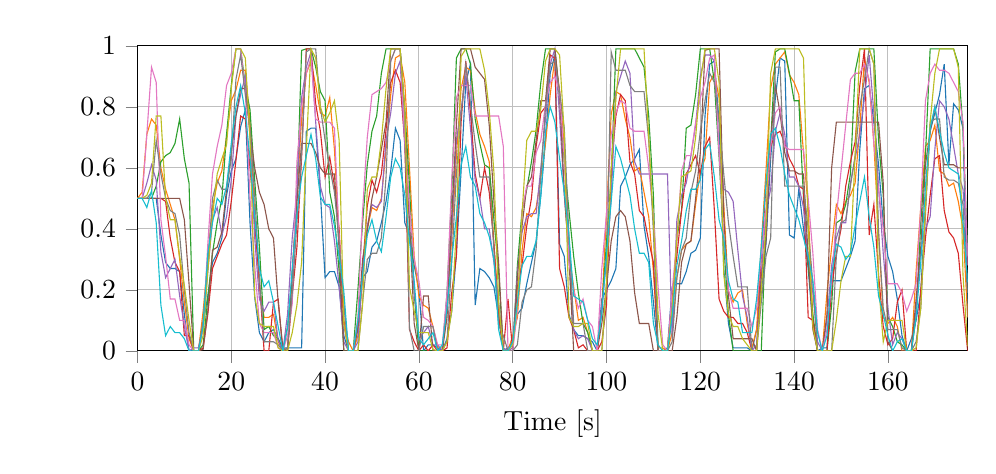
\begin{tikzpicture}

\definecolor{color1}{rgb}{1,0.498039215686275,0.0549019607843137}
\definecolor{color0}{rgb}{0.12156862745098,0.466666666666667,0.705882352941177}
\definecolor{color3}{rgb}{0.83921568627451,0.152941176470588,0.156862745098039}
\definecolor{color2}{rgb}{0.172549019607843,0.627450980392157,0.172549019607843}
\definecolor{color5}{rgb}{0.549019607843137,0.337254901960784,0.294117647058824}
\definecolor{color4}{rgb}{0.580392156862745,0.403921568627451,0.741176470588235}
\definecolor{color7}{rgb}{0.737254901960784,0.741176470588235,0.133333333333333}
\definecolor{color6}{rgb}{0.890196078431372,0.466666666666667,0.76078431372549}
\definecolor{color8}{rgb}{0.0901960784313725,0.745098039215686,0.811764705882353}

\begin{axis}[
width=\textwidth,
height=0.45\textwidth,
xlabel={Time [s]},
ylabel={\phantom{Green intensity value}},
xmin=0, xmax=177,
ymin=0, ymax=1,
tick align=outside,
tick pos=left,
xmajorgrids,
ymajorgrids,
]
\addplot [thin, color0, forget plot]
table {%
0 0.5
1 0.5
2 0.5
3 0.5
4 0.5
4.99999999999999 0.38
5.99999999999999 0.29
6.99999999999998 0.27
7.99999999999998 0.27
8.99999999999998 0.26
9.99999999999998 0.12
11 0
12 0
13 0
14 0.09
15 0.18
16 0.29
17 0.32
18 0.37
19.0000000000001 0.51
20.0000000000002 0.59
21.0000000000002 0.63
22.0000000000002 0.735
23.0000000000003 0.79
24.0000000000004 0.42
25.0000000000004 0.175
26.0000000000004 0.06
27.0000000000005 0.03
28.0000000000006 0.06
29.0000000000006 0.07
30.0000000000007 0.04
31.0000000000007 0.01
32.0000000000007 0.01
33.0000000000007 0.01
34.0000000000006 0.01
35.0000000000006 0.01
36.0000000000005 0.72
37.0000000000005 0.73
38.0000000000004 0.73
39.0000000000003 0.52
40.0000000000003 0.24
41.0000000000002 0.26
42.0000000000002 0.26
43.0000000000001 0.21
44.0000000000001 0.05
45 0
46 0
46.9999999999999 0.07
47.9999999999999 0.24
48.9999999999998 0.26
49.9999999999997 0.34
50.9999999999997 0.36
51.9999999999996 0.42
52.9999999999995 0.49
53.9999999999995 0.59
54.9999999999994 0.73
55.9999999999994 0.69
56.9999999999993 0.42
57.9999999999993 0.38
58.9999999999992 0.28
59.9999999999992 0.2
60.9999999999991 0
61.999999999999 0.02
62.999999999999 0.02
63.9999999999989 0.01
64.9999999999989 0
65.9999999999988 0.04
66.9999999999988 0.13
67.9999999999987 0.32
68.9999999999986 0.59
69.9999999999986 0.88
70.9999999999986 0.94
71.9999999999985 0.15
72.9999999999984 0.27
73.9999999999984 0.26
74.9999999999983 0.24
75.9999999999983 0.21
76.9999999999982 0.11
77.9999999999981 0
78.9999999999981 0.01
79.999999999998 0.03
80.999999999998 0.12
81.9999999999979 0.14
82.9999999999979 0.22
83.9999999999978 0.29
84.9999999999977 0.36
85.9999999999977 0.51
86.9999999999976 0.69
87.9999999999976 0.91
88.9999999999975 0.97
89.9999999999974 0.35
90.9999999999974 0.31
91.9999999999973 0.12
92.9999999999973 0.07
93.9999999999972 0.05
94.9999999999972 0.05
95.9999999999971 0.04
96.9999999999971 0.03
97.999999999997 0
98.9999999999969 0.17
99.9999999999969 0.2
100.999999999997 0.23
101.999999999997 0.27
102.999999999997 0.54
103.999999999997 0.57
104.999999999997 0.61
105.999999999997 0.63
106.999999999996 0.66
107.999999999996 0.41
108.999999999996 0.31
109.999999999996 0.16
110.999999999996 0
111.999999999996 0
112.999999999996 0.01
113.999999999996 0.21
114.999999999996 0.22
115.999999999996 0.22
116.999999999996 0.26
117.999999999996 0.32
118.999999999996 0.33
119.999999999996 0.37
120.999999999996 0.77
121.999999999996 0.94
122.999999999996 0.95
123.999999999996 0.75
124.999999999995 0.27
125.999999999995 0.09
126.999999999995 0.01
127.999999999995 0.01
128.999999999995 0.01
129.999999999995 0.01
130.999999999995 0
131.999999999995 0.07
132.999999999995 0.19
133.999999999995 0.35
134.999999999995 0.63
135.999999999995 0.83
136.999999999995 0.96
137.999999999995 0.95
138.999999999995 0.38
139.999999999995 0.37
140.999999999995 0.53
141.999999999995 0.4
142.999999999994 0.27
143.999999999994 0.08
144.999999999994 0
145.999999999994 0.01
146.999999999994 0.01
147.999999999994 0.23
148.999999999994 0.23
149.999999999994 0.23
150.999999999994 0.27
151.999999999994 0.31
152.999999999994 0.36
153.999999999994 0.66
154.999999999994 0.86
155.999999999994 0.87
156.999999999994 0.75
157.999999999994 0.61
158.999999999994 0.42
159.999999999993 0.31
160.999999999993 0.26
161.999999999993 0.17
162.999999999993 0.05
163.999999999993 0
164.999999999993 0.04
165.999999999993 0.1
166.999999999993 0.19
167.999999999993 0.48
168.999999999993 0.72
169.999999999993 0.78
170.999999999993 0.84
171.999999999993 0.94
172.999999999993 0.61
173.999999999993 0.81
174.999999999993 0.79
175.999999999993 0.73
176.999999999993 0.11
};
\addplot [thin, color1, forget plot]
table {%
0 0.5
1 0.52
2 0.71
3 0.76
4 0.74
4.99999999999999 0.6
5.99999999999999 0.53
6.99999999999998 0.48
7.99999999999998 0.43
8.99999999999998 0.3
9.99999999999998 0.16
11 0.04
12 0
13 0
14 0.13
15 0.3
16 0.47
17 0.55
18 0.59
19.0000000000001 0.705
20.0000000000002 0.82
21.0000000000002 0.855
22.0000000000002 0.92
23.0000000000003 0.92
24.0000000000004 0.75
25.0000000000004 0.45
26.0000000000004 0.21
27.0000000000005 0.11
28.0000000000006 0.11
29.0000000000006 0.12
30.0000000000007 0.03
31.0000000000007 0
32.0000000000007 0.01
33.0000000000007 0.25
34.0000000000006 0.51
35.0000000000006 0.76
36.0000000000005 0.91
37.0000000000005 0.95
38.0000000000004 0.87
39.0000000000003 0.78
40.0000000000003 0.77
41.0000000000002 0.83
42.0000000000002 0.66
43.0000000000001 0.37
44.0000000000001 0.1
45 0.03
46 0
46.9999999999999 0.05
47.9999999999999 0.24
48.9999999999998 0.4
49.9999999999997 0.47
50.9999999999997 0.46
51.9999999999996 0.5
52.9999999999995 0.66
53.9999999999995 0.84
54.9999999999994 0.96
55.9999999999994 0.97
56.9999999999993 0.88
57.9999999999993 0.6
58.9999999999992 0.31
59.9999999999992 0.18
60.9999999999991 0.15
61.999999999999 0.14
62.999999999999 0.08
63.9999999999989 0.01
64.9999999999989 0.01
65.9999999999988 0.13
66.9999999999988 0.37
67.9999999999987 0.64
68.9999999999986 0.86
69.9999999999986 0.93
70.9999999999986 0.92
71.9999999999985 0.785
72.9999999999984 0.71
73.9999999999984 0.67
74.9999999999983 0.62
75.9999999999983 0.35
76.9999999999982 0.13
77.9999999999981 0
78.9999999999981 0
79.999999999998 0.05
80.999999999998 0.11
81.9999999999979 0.33
82.9999999999979 0.45
83.9999999999978 0.44
84.9999999999977 0.47
85.9999999999977 0.57
86.9999999999976 0.68
87.9999999999976 0.84
88.9999999999975 0.96
89.9999999999974 0.855
90.9999999999974 0.67
91.9999999999973 0.32
92.9999999999973 0.21
93.9999999999972 0.1
94.9999999999972 0.11
95.9999999999971 0.06
96.9999999999971 0
97.999999999997 0
98.9999999999969 0.14
99.9999999999969 0.45
100.999999999997 0.775
101.999999999997 0.85
102.999999999997 0.84
103.999999999997 0.76
104.999999999997 0.7
105.999999999997 0.59
106.999999999996 0.6
107.999999999996 0.52
108.999999999996 0.44
109.999999999996 0.26
110.999999999996 0.01
111.999999999996 0.01
112.999999999996 0
113.999999999996 0.06
114.999999999996 0.24
115.999999999996 0.33
116.999999999996 0.35
117.999999999996 0.36
118.999999999996 0.48
119.999999999996 0.59
120.999999999996 0.63
121.999999999996 0.88
122.999999999996 0.91
123.999999999996 0.83
124.999999999995 0.48
125.999999999995 0.195
126.999999999995 0.16
127.999999999995 0.19
128.999999999995 0.2
129.999999999995 0.09
130.999999999995 0.01
131.999999999995 0.07
132.999999999995 0.35
133.999999999995 0.59
134.999999999995 0.86
135.999999999995 0.94
136.999999999995 0.96
137.999999999995 0.98
138.999999999995 0.905
139.999999999995 0.88
140.999999999995 0.84
141.999999999995 0.65
142.999999999994 0.47
143.999999999994 0.1
144.999999999994 0
145.999999999994 0
146.999999999994 0.19
147.999999999994 0.34
148.999999999994 0.48
149.999999999994 0.45
150.999999999994 0.49
151.999999999994 0.51
152.999999999994 0.55
153.999999999994 0.73
154.999999999994 0.96
155.999999999994 0.88
156.999999999994 0.68
157.999999999994 0.39
158.999999999994 0.11
159.999999999993 0.09
160.999999999993 0.11
161.999999999993 0.08
162.999999999993 0
163.999999999993 0
164.999999999993 0
165.999999999993 0.26
166.999999999993 0.47
167.999999999993 0.67
168.999999999993 0.69
169.999999999993 0.74
170.999999999993 0.59
171.999999999993 0.58
172.999999999993 0.54
173.999999999993 0.55
174.999999999993 0.49
175.999999999993 0.4
176.999999999993 0.11
};
\addplot [thin, color2, forget plot]
table {%
0 0.5
1 0.5
2 0.5
3 0.5
4 0.54
4.99999999999999 0.62
5.99999999999999 0.64
6.99999999999998 0.65
7.99999999999998 0.68
8.99999999999998 0.76
9.99999999999998 0.63
11 0.55
12 0
13 0
14 0.02
15 0.17
16 0.32
17 0.42
18 0.5
19.0000000000001 0.71
20.0000000000002 0.87
21.0000000000002 0.99
22.0000000000002 0.99
23.0000000000003 0.87
24.0000000000004 0.79
25.0000000000004 0.56
26.0000000000004 0.34
27.0000000000005 0.07
28.0000000000006 0.08
29.0000000000006 0.05
30.0000000000007 0.04
31.0000000000007 0
32.0000000000007 0.08
33.0000000000007 0.24
34.0000000000006 0.505
35.0000000000006 0.985
36.0000000000005 0.99
37.0000000000005 0.99
38.0000000000004 0.93
39.0000000000003 0.85
40.0000000000003 0.82
41.0000000000002 0.52
42.0000000000002 0.44
43.0000000000001 0.26
44.0000000000001 0
45 0
46 0
46.9999999999999 0.2
47.9999999999999 0.42
48.9999999999998 0.61
49.9999999999997 0.72
50.9999999999997 0.77
51.9999999999996 0.91
52.9999999999995 0.99
53.9999999999995 0.99
54.9999999999994 0.99
55.9999999999994 0.99
56.9999999999993 0.79
57.9999999999993 0.54
58.9999999999992 0.19
59.9999999999992 0
60.9999999999991 0
61.999999999999 0
62.999999999999 0
63.9999999999989 0
64.9999999999989 0
65.9999999999988 0.19
66.9999999999988 0.52
67.9999999999987 0.96
68.9999999999986 0.99
69.9999999999986 0.99
70.9999999999986 0.94
71.9999999999985 0.76
72.9999999999984 0.68
73.9999999999984 0.61
74.9999999999983 0.6
75.9999999999983 0.43
76.9999999999982 0.26
77.9999999999981 0
78.9999999999981 0
79.999999999998 0
80.999999999998 0.28
81.9999999999979 0.46
82.9999999999979 0.53
83.9999999999978 0.62
84.9999999999977 0.725
85.9999999999977 0.88
86.9999999999976 0.99
87.9999999999976 0.99
88.9999999999975 0.99
89.9999999999974 0.83
90.9999999999974 0.62
91.9999999999973 0.46
92.9999999999973 0.31
93.9999999999972 0.19
94.9999999999972 0.09
95.9999999999971 0.06
96.9999999999971 0
97.999999999997 0
98.9999999999969 0.14
99.9999999999969 0.355
100.999999999997 0.565
101.999999999997 0.99
102.999999999997 0.99
103.999999999997 0.99
104.999999999997 0.99
105.999999999997 0.99
106.999999999996 0.96
107.999999999996 0.93
108.999999999996 0.77
109.999999999996 0.51
110.999999999996 0
111.999999999996 0
112.999999999996 0
113.999999999996 0.11
114.999999999996 0.37
115.999999999996 0.46
116.999999999996 0.73
117.999999999996 0.74
118.999999999996 0.84
119.999999999996 0.99
120.999999999996 0.99
121.999999999996 0.99
122.999999999996 0.88
123.999999999996 0.635
124.999999999995 0.35
125.999999999995 0.12
126.999999999995 0
127.999999999995 0
128.999999999995 0
129.999999999995 0
130.999999999995 0
131.999999999995 0
132.999999999995 0
133.999999999995 0.425
134.999999999995 0.68
135.999999999995 0.98
136.999999999995 0.99
137.999999999995 0.99
138.999999999995 0.91
139.999999999995 0.82
140.999999999995 0.82
141.999999999995 0.5
142.999999999994 0.28
143.999999999994 0.12
144.999999999994 0
145.999999999994 0
146.999999999994 0
147.999999999994 0.15
148.999999999994 0.42
149.999999999994 0.43
150.999999999994 0.48
151.999999999994 0.58
152.999999999994 0.915
153.999999999994 0.99
154.999999999994 0.99
155.999999999994 0.99
156.999999999994 0.99
157.999999999994 0.69
158.999999999994 0.51
159.999999999993 0.11
160.999999999993 0.08
161.999999999993 0.03
162.999999999993 0.02
163.999999999993 0
164.999999999993 0
165.999999999993 0.11
166.999999999993 0.42
167.999999999993 0.64
168.999999999993 0.99
169.999999999993 0.99
170.999999999993 0.99
171.999999999993 0.99
172.999999999993 0.99
173.999999999993 0.99
174.999999999993 0.94
175.999999999993 0.73
176.999999999993 0.315
};
\addplot [thin, color3, forget plot]
table {%
0 0.5
1 0.5
2 0.5
3 0.5
4 0.5
4.99999999999999 0.5
5.99999999999999 0.49
6.99999999999998 0.37
7.99999999999998 0.29
8.99999999999998 0.26
9.99999999999998 0.05
11 0.05
12 0
13 0
14 0.01
15 0.12
16 0.27
17 0.31
18 0.35
19.0000000000001 0.38
20.0000000000002 0.49
21.0000000000002 0.625
22.0000000000002 0.77
23.0000000000003 0.76
24.0000000000004 0.6
25.0000000000004 0.42
26.0000000000004 0.23
27.0000000000005 0
28.0000000000006 0
29.0000000000006 0.16
30.0000000000007 0.17
31.0000000000007 0
32.0000000000007 0
33.0000000000007 0.18
34.0000000000006 0.34
35.0000000000006 0.635
36.0000000000005 0.99
37.0000000000005 0.99
38.0000000000004 0.81
39.0000000000003 0.72
40.0000000000003 0.57
41.0000000000002 0.635
42.0000000000002 0.54
43.0000000000001 0.4
44.0000000000001 0.09
45 0
46 0
46.9999999999999 0.08
47.9999999999999 0.27
48.9999999999998 0.475
49.9999999999997 0.56
50.9999999999997 0.52
51.9999999999996 0.58
52.9999999999995 0.725
53.9999999999995 0.88
54.9999999999994 0.92
55.9999999999994 0.88
56.9999999999993 0.68
57.9999999999993 0.07
58.9999999999992 0.03
59.9999999999992 0
60.9999999999991 0.02
61.999999999999 0
62.999999999999 0.02
63.9999999999989 0
64.9999999999989 0
65.9999999999988 0.01
66.9999999999988 0.19
67.9999999999987 0.31
68.9999999999986 0.75
69.9999999999986 0.95
70.9999999999986 0.78
71.9999999999985 0.58
72.9999999999984 0.5
73.9999999999984 0.6
74.9999999999983 0.52
75.9999999999983 0.35
76.9999999999982 0.12
77.9999999999981 0
78.9999999999981 0.17
79.999999999998 0
80.999999999998 0.21
81.9999999999979 0.28
82.9999999999979 0.41
83.9999999999978 0.5
84.9999999999977 0.67
85.9999999999977 0.78
86.9999999999976 0.8
87.9999999999976 0.97
88.9999999999975 0.96
89.9999999999974 0.27
90.9999999999974 0.21
91.9999999999973 0.11
92.9999999999973 0.07
93.9999999999972 0.01
94.9999999999972 0.02
95.9999999999971 0
96.9999999999971 0
97.999999999997 0
98.9999999999969 0.03
99.9999999999969 0.15
100.999999999997 0.59
101.999999999997 0.77
102.999999999997 0.84
103.999999999997 0.82
104.999999999997 0.62
105.999999999997 0.58
106.999999999996 0.46
107.999999999996 0.44
108.999999999996 0.36
109.999999999996 0.29
110.999999999996 0
111.999999999996 0
112.999999999996 0
113.999999999996 0.18
114.999999999996 0.31
115.999999999996 0.46
116.999999999996 0.58
117.999999999996 0.61
118.999999999996 0.64
119.999999999996 0.58
120.999999999996 0.67
121.999999999996 0.7
122.999999999996 0.46
123.999999999996 0.17
124.999999999995 0.13
125.999999999995 0.11
126.999999999995 0.11
127.999999999995 0.09
128.999999999995 0.09
129.999999999995 0.06
130.999999999995 0
131.999999999995 0
132.999999999995 0.31
133.999999999995 0.54
134.999999999995 0.67
135.999999999995 0.71
136.999999999995 0.72
137.999999999995 0.68
138.999999999995 0.63
139.999999999995 0.6
140.999999999995 0.54
141.999999999995 0.53
142.999999999994 0.11
143.999999999994 0.1
144.999999999994 0
145.999999999994 0
146.999999999994 0
147.999999999994 0.21
148.999999999994 0.32
149.999999999994 0.4
150.999999999994 0.54
151.999999999994 0.62
152.999999999994 0.685
153.999999999994 0.87
154.999999999994 0.99
155.999999999994 0.38
156.999999999994 0.48
157.999999999994 0.25
158.999999999994 0.08
159.999999999993 0.02
160.999999999993 0.04
161.999999999993 0.16
162.999999999993 0.2
163.999999999993 0
164.999999999993 0
165.999999999993 0
166.999999999993 0.2
167.999999999993 0.37
168.999999999993 0.51
169.999999999993 0.63
170.999999999993 0.64
171.999999999993 0.46
172.999999999993 0.39
173.999999999993 0.37
174.999999999993 0.32
175.999999999993 0.15
176.999999999993 0
};
\addplot [thin, color4, forget plot]
table {%
0 0.5
1 0.5
2 0.55
3 0.61
4 0.56
4.99999999999999 0.325
5.99999999999999 0.24
6.99999999999998 0.27
7.99999999999998 0.3
8.99999999999998 0.18
9.99999999999998 0.08
11 0
12 0.01
13 0.01
14 0.08
15 0.26
16 0.43
17 0.47
18 0.38
19.0000000000001 0.44
20.0000000000002 0.56
21.0000000000002 0.77
22.0000000000002 0.84
23.0000000000003 0.9
24.0000000000004 0.7
25.0000000000004 0.37
26.0000000000004 0.17
27.0000000000005 0.13
28.0000000000006 0.16
29.0000000000006 0.16
30.0000000000007 0.035
31.0000000000007 0
32.0000000000007 0.12
33.0000000000007 0.37
34.0000000000006 0.52
35.0000000000006 0.83
36.0000000000005 0.93
37.0000000000005 0.98
38.0000000000004 0.75
39.0000000000003 0.54
40.0000000000003 0.48
41.0000000000002 0.47
42.0000000000002 0.36
43.0000000000001 0.21
44.0000000000001 0.03
45 0
46 0
46.9999999999999 0.03
47.9999999999999 0.265
48.9999999999998 0.41
49.9999999999997 0.48
50.9999999999997 0.47
51.9999999999996 0.49
52.9999999999995 0.69
53.9999999999995 0.78
54.9999999999994 0.91
55.9999999999994 0.95
56.9999999999993 0.67
57.9999999999993 0.41
58.9999999999992 0.2
59.9999999999992 0.04
60.9999999999991 0.06
61.999999999999 0.08
62.999999999999 0.02
63.9999999999989 0.02
64.9999999999989 0
65.9999999999988 0.175
66.9999999999988 0.4
67.9999999999987 0.69
68.9999999999986 0.79
69.9999999999986 0.9
70.9999999999986 0.73
71.9999999999985 0.56
72.9999999999984 0.5
73.9999999999984 0.4
74.9999999999983 0.4
75.9999999999983 0.29
76.9999999999982 0.16
77.9999999999981 0.01
78.9999999999981 0
79.999999999998 0.01
80.999999999998 0.26
81.9999999999979 0.39
82.9999999999979 0.44
83.9999999999978 0.45
84.9999999999977 0.45
85.9999999999977 0.6
86.9999999999976 0.76
87.9999999999976 0.94
88.9999999999975 0.99
89.9999999999974 0.77
90.9999999999974 0.51
91.9999999999973 0.32
92.9999999999973 0.07
93.9999999999972 0.04
94.9999999999972 0.05
95.9999999999971 0.04
96.9999999999971 0
97.999999999997 0
98.9999999999969 0.15
99.9999999999969 0.29
100.999999999997 0.5
101.999999999997 0.85
102.999999999997 0.9
103.999999999997 0.95
104.999999999997 0.91
105.999999999997 0.62
106.999999999996 0.58
107.999999999996 0.58
108.999999999996 0.58
109.999999999996 0.58
110.999999999996 0.58
111.999999999996 0.58
112.999999999996 0.58
113.999999999996 0.04
114.999999999996 0.43
115.999999999996 0.51
116.999999999996 0.55
117.999999999996 0.64
118.999999999996 0.74
119.999999999996 0.9
120.999999999996 0.97
121.999999999996 0.97
122.999999999996 0.95
123.999999999996 0.65
124.999999999995 0.53
125.999999999995 0.52
126.999999999995 0.49
127.999999999995 0.33
128.999999999995 0.18
129.999999999995 0.11
130.999999999995 0
131.999999999995 0.02
132.999999999995 0.25
133.999999999995 0.46
134.999999999995 0.53
135.999999999995 0.72
136.999999999995 0.78
137.999999999995 0.71
138.999999999995 0.57
139.999999999995 0.57
140.999999999995 0.54
141.999999999995 0.47
142.999999999994 0.3
143.999999999994 0.19
144.999999999994 0.03
145.999999999994 0
146.999999999994 0.1
147.999999999994 0.28
148.999999999994 0.37
149.999999999994 0.42
150.999999999994 0.42
151.999999999994 0.55
152.999999999994 0.63
153.999999999994 0.71
154.999999999994 0.83
155.999999999994 0.97
156.999999999994 0.78
157.999999999994 0.54
158.999999999994 0.32
159.999999999993 0.14
160.999999999993 0.02
161.999999999993 0.06
162.999999999993 0.04
163.999999999993 0
164.999999999993 0
165.999999999993 0.14
166.999999999993 0.33
167.999999999993 0.4
168.999999999993 0.44
169.999999999993 0.66
170.999999999993 0.82
171.999999999993 0.8
172.999999999993 0.76
173.999999999993 0.67
174.999999999993 0.58
175.999999999993 0.53
176.999999999993 0.31
};
\addplot [thin, color5, forget plot]
table {%
0 0.5
1 0.5
2 0.5
3 0.5
4 0.5
4.99999999999999 0.5
5.99999999999999 0.5
6.99999999999998 0.5
7.99999999999998 0.5
8.99999999999998 0.5
9.99999999999998 0.43
11 0.22
12 0
13 0
14 0.005
15 0.13
16 0.33
17 0.34
18 0.39
19.0000000000001 0.53
20.0000000000002 0.65
21.0000000000002 0.77
22.0000000000002 0.86
23.0000000000003 0.86
24.0000000000004 0.72
25.0000000000004 0.6
26.0000000000004 0.52
27.0000000000005 0.48
28.0000000000006 0.4
29.0000000000006 0.37
30.0000000000007 0.16
31.0000000000007 0.01
32.0000000000007 0
33.0000000000007 0.26
34.0000000000006 0.49
35.0000000000006 0.68
36.0000000000005 0.68
37.0000000000005 0.68
38.0000000000004 0.65
39.0000000000003 0.6
40.0000000000003 0.58
41.0000000000002 0.58
42.0000000000002 0.58
43.0000000000001 0.33
44.0000000000001 0
45 0
46 0
46.9999999999999 0.08
47.9999999999999 0.3
48.9999999999998 0.395
49.9999999999997 0.5
50.9999999999997 0.57
51.9999999999996 0.66
52.9999999999995 0.75
53.9999999999995 0.99
54.9999999999994 0.99
55.9999999999994 0.99
56.9999999999993 0.78
57.9999999999993 0.42
58.9999999999992 0.09
59.9999999999992 0
60.9999999999991 0.18
61.999999999999 0.18
62.999999999999 0
63.9999999999989 0
64.9999999999989 0
65.9999999999988 0.11
66.9999999999988 0.44
67.9999999999987 0.74
68.9999999999986 0.99
69.9999999999986 0.99
70.9999999999986 0.99
71.9999999999985 0.93
72.9999999999984 0.91
73.9999999999984 0.89
74.9999999999983 0.74
75.9999999999983 0.49
76.9999999999982 0.29
77.9999999999981 0
78.9999999999981 0
79.999999999998 0
80.999999999998 0.24
81.9999999999979 0.41
82.9999999999979 0.54
83.9999999999978 0.57
84.9999999999977 0.69
85.9999999999977 0.82
86.9999999999976 0.82
87.9999999999976 0.99
88.9999999999975 0.99
89.9999999999974 0.84
90.9999999999974 0.52
91.9999999999973 0.3
92.9999999999973 0
93.9999999999972 0
94.9999999999972 0
95.9999999999971 0
96.9999999999971 0
97.999999999997 0
98.9999999999969 0.09
99.9999999999969 0.21
100.999999999997 0.36
101.999999999997 0.44
102.999999999997 0.46
103.999999999997 0.44
104.999999999997 0.36
105.999999999997 0.19
106.999999999996 0.09
107.999999999996 0.09
108.999999999996 0.09
109.999999999996 0
110.999999999996 0
111.999999999996 0
112.999999999996 0
113.999999999996 0
114.999999999996 0.11
115.999999999996 0.29
116.999999999996 0.35
117.999999999996 0.36
118.999999999996 0.5
119.999999999996 0.65
120.999999999996 0.985
121.999999999996 0.99
122.999999999996 0.99
123.999999999996 0.99
124.999999999995 0.44
125.999999999995 0.18
126.999999999995 0.04
127.999999999995 0.04
128.999999999995 0.04
129.999999999995 0.04
130.999999999995 0.04
131.999999999995 0
132.999999999995 0.24
133.999999999995 0.36
134.999999999995 0.69
135.999999999995 0.87
136.999999999995 0.78
137.999999999995 0.65
138.999999999995 0.59
139.999999999995 0.59
140.999999999995 0.58
141.999999999995 0.58
142.999999999994 0.31
143.999999999994 0.07
144.999999999994 0
145.999999999994 0
146.999999999994 0.12
147.999999999994 0.6
148.999999999994 0.75
149.999999999994 0.75
150.999999999994 0.75
151.999999999994 0.75
152.999999999994 0.75
153.999999999994 0.75
154.999999999994 0.75
155.999999999994 0.75
156.999999999994 0.75
157.999999999994 0.75
158.999999999994 0.55
159.999999999993 0.03
160.999999999993 0
161.999999999993 0
162.999999999993 0
163.999999999993 0
164.999999999993 0
165.999999999993 0.17
166.999999999993 0.34
167.999999999993 0.61
168.999999999993 0.72
169.999999999993 0.8
170.999999999993 0.7
171.999999999993 0.61
172.999999999993 0.61
173.999999999993 0.61
174.999999999993 0.6
175.999999999993 0.6
176.999999999993 0.6
};
\addplot [thin, color6, forget plot]
table {%
0 0.5
1 0.5
2 0.71
3 0.93
4 0.88
4.99999999999999 0.43
5.99999999999999 0.31
6.99999999999998 0.17
7.99999999999998 0.17
8.99999999999998 0.1
9.99999999999998 0.1
11 0.02
12 0
13 0
14 0.07
15 0.35
16 0.58
17 0.67
18 0.74
19.0000000000001 0.87
20.0000000000002 0.91
21.0000000000002 0.99
22.0000000000002 0.99
23.0000000000003 0.85
24.0000000000004 0.5
25.0000000000004 0.28
26.0000000000004 0.09
27.0000000000005 0.06
28.0000000000006 0.06
29.0000000000006 0.06
30.0000000000007 0.01
31.0000000000007 0
32.0000000000007 0.05
33.0000000000007 0.155
34.0000000000006 0.62
35.0000000000006 0.8
36.0000000000005 0.91
37.0000000000005 0.96
38.0000000000004 0.76
39.0000000000003 0.75
40.0000000000003 0.75
41.0000000000002 0.75
42.0000000000002 0.73
43.0000000000001 0.37
44.0000000000001 0.16
45 0
46 0
46.9999999999999 0.11
47.9999999999999 0.46
48.9999999999998 0.7
49.9999999999997 0.84
50.9999999999997 0.85
51.9999999999996 0.86
52.9999999999995 0.88
53.9999999999995 0.95
54.9999999999994 0.99
55.9999999999994 0.99
56.9999999999993 0.69
57.9999999999993 0.47
58.9999999999992 0.3
59.9999999999992 0.23
60.9999999999991 0.11
61.999999999999 0.1
62.999999999999 0.08
63.9999999999989 0.02
64.9999999999989 0.02
65.9999999999988 0.19
66.9999999999988 0.56
67.9999999999987 0.83
68.9999999999986 0.87
69.9999999999986 0.87
70.9999999999986 0.87
71.9999999999985 0.77
72.9999999999984 0.77
73.9999999999984 0.77
74.9999999999983 0.77
75.9999999999983 0.77
76.9999999999982 0.77
77.9999999999981 0.67
78.9999999999981 0
79.999999999998 0
80.999999999998 0.13
81.9999999999979 0.46
82.9999999999979 0.54
83.9999999999978 0.54
84.9999999999977 0.65
85.9999999999977 0.69
86.9999999999976 0.81
87.9999999999976 0.88
88.9999999999975 0.9
89.9999999999974 0.85
90.9999999999974 0.63
91.9999999999973 0.29
92.9999999999973 0.2
93.9999999999972 0.14
94.9999999999972 0.17
95.9999999999971 0.1
96.9999999999971 0.08
97.999999999997 0
98.9999999999969 0.27
99.9999999999969 0.45
100.999999999997 0.71
101.999999999997 0.78
102.999999999997 0.82
103.999999999997 0.81
104.999999999997 0.73
105.999999999997 0.72
106.999999999996 0.72
107.999999999996 0.72
108.999999999996 0.6
109.999999999996 0.44
110.999999999996 0.21
111.999999999996 0.02
112.999999999996 0
113.999999999996 0.2
114.999999999996 0.36
115.999999999996 0.59
116.999999999996 0.64
117.999999999996 0.64
118.999999999996 0.75
119.999999999996 0.83
120.999999999996 0.88
121.999999999996 0.96
122.999999999996 0.97
123.999999999996 0.65
124.999999999995 0.37
125.999999999995 0.2
126.999999999995 0.14
127.999999999995 0.14
128.999999999995 0.14
129.999999999995 0.14
130.999999999995 0.08
131.999999999995 0.14
132.999999999995 0.32
133.999999999995 0.46
134.999999999995 0.67
135.999999999995 0.78
136.999999999995 0.8
137.999999999995 0.67
138.999999999995 0.66
139.999999999995 0.66
140.999999999995 0.66
141.999999999995 0.66
142.999999999994 0.5
143.999999999994 0.32
144.999999999994 0.07
145.999999999994 0
146.999999999994 0.07
147.999999999994 0.22
148.999999999994 0.44
149.999999999994 0.59
150.999999999994 0.74
151.999999999994 0.89
152.999999999994 0.91
153.999999999994 0.91
154.999999999994 0.94
155.999999999994 0.89
156.999999999994 0.68
157.999999999994 0.53
158.999999999994 0.4
159.999999999993 0.22
160.999999999993 0.22
161.999999999993 0.22
162.999999999993 0.19
163.999999999993 0.13
164.999999999993 0.17
165.999999999993 0.22
166.999999999993 0.47
167.999999999993 0.82
168.999999999993 0.91
169.999999999993 0.94
170.999999999993 0.92
171.999999999993 0.92
172.999999999993 0.91
173.999999999993 0.88
174.999999999993 0.85
175.999999999993 0.75
176.999999999993 0.28
};
\addplot [thin, lightgray!66.405228758169926!black, forget plot]
table {%
0 0.5
1 0.5
2 0.5
3 0.52
4 0.69
4.99999999999999 0.58
5.99999999999999 0.5
6.99999999999998 0.46
7.99999999999998 0.45
8.99999999999998 0.38
9.99999999999998 0.2
11 0.06
12 0
13 0
14 0.1
15 0.28
16 0.5
17 0.56
18 0.53
19.0000000000001 0.53
20.0000000000002 0.63
21.0000000000002 0.89
22.0000000000002 0.97
23.0000000000003 0.84
24.0000000000004 0.73
25.0000000000004 0.51
26.0000000000004 0.24
27.0000000000005 0.03
28.0000000000006 0.03
29.0000000000006 0.03
30.0000000000007 0.02
31.0000000000007 0
32.0000000000007 0.01
33.0000000000007 0.19
34.0000000000006 0.42
35.0000000000006 0.65
36.0000000000005 0.98
37.0000000000005 0.99
38.0000000000004 0.99
39.0000000000003 0.8
40.0000000000003 0.69
41.0000000000002 0.6
42.0000000000002 0.52
43.0000000000001 0.36
44.0000000000001 0.15
45 0
46 0
46.9999999999999 0
47.9999999999999 0.16
48.9999999999998 0.3
49.9999999999997 0.32
50.9999999999997 0.32
51.9999999999996 0.37
52.9999999999995 0.57
53.9999999999995 0.95
54.9999999999994 0.99
55.9999999999994 0.99
56.9999999999993 0.77
57.9999999999993 0.075
58.9999999999992 0
59.9999999999992 0
60.9999999999991 0.08
61.999999999999 0.08
62.999999999999 0.08
63.9999999999989 0
64.9999999999989 0
65.9999999999988 0.035
66.9999999999988 0.29
67.9999999999987 0.58
68.9999999999986 0.775
69.9999999999986 0.94
70.9999999999986 0.81
71.9999999999985 0.68
72.9999999999984 0.57
73.9999999999984 0.57
74.9999999999983 0.57
75.9999999999983 0.33
76.9999999999982 0.085
77.9999999999981 0.05
78.9999999999981 0
79.999999999998 0
80.999999999998 0.02
81.9999999999979 0.16
82.9999999999979 0.2
83.9999999999978 0.21
84.9999999999977 0.335
85.9999999999977 0.58
86.9999999999976 0.8
87.9999999999976 0.94
88.9999999999975 0.95
89.9999999999974 0.85
90.9999999999974 0.73
91.9999999999973 0.37
92.9999999999973 0.09
93.9999999999972 0.09
94.9999999999972 0.09
95.9999999999971 0
96.9999999999971 0
97.999999999997 0
98.9999999999969 0
99.9999999999969 0.21
100.999999999997 0.98
101.999999999997 0.92
102.999999999997 0.92
103.999999999997 0.92
104.999999999997 0.87
105.999999999997 0.85
106.999999999996 0.85
107.999999999996 0.85
108.999999999996 0.69
109.999999999996 0.39
110.999999999996 0
111.999999999996 0
112.999999999996 0
113.999999999996 0.03
114.999999999996 0.24
115.999999999996 0.33
116.999999999996 0.37
117.999999999996 0.52
118.999999999996 0.59
119.999999999996 0.72
120.999999999996 0.82
121.999999999996 0.91
122.999999999996 0.88
123.999999999996 0.755
124.999999999995 0.58
125.999999999995 0.42
126.999999999995 0.31
127.999999999995 0.21
128.999999999995 0.21
129.999999999995 0.21
130.999999999995 0
131.999999999995 0
132.999999999995 0.16
133.999999999995 0.31
134.999999999995 0.37
135.999999999995 0.93
136.999999999995 0.93
137.999999999995 0.54
138.999999999995 0.54
139.999999999995 0.54
140.999999999995 0.54
141.999999999995 0.54
142.999999999994 0.4
143.999999999994 0.22
144.999999999994 0
145.999999999994 0
146.999999999994 0
147.999999999994 0
148.999999999994 0.31
149.999999999994 0.42
150.999999999994 0.43
151.999999999994 0.54
152.999999999994 0.64
153.999999999994 0.8
154.999999999994 0.89
155.999999999994 0.99
156.999999999994 0.94
157.999999999994 0.39
158.999999999994 0.14
159.999999999993 0.07
160.999999999993 0.07
161.999999999993 0.07
162.999999999993 0.01
163.999999999993 0
164.999999999993 0
165.999999999993 0.03
166.999999999993 0.14
167.999999999993 0.445
168.999999999993 0.75
169.999999999993 0.76
170.999999999993 0.76
171.999999999993 0.57
172.999999999993 0.56
173.999999999993 0.56
174.999999999993 0.55
175.999999999993 0.48
176.999999999993 0.19
};
\addplot [thin, color7, forget plot]
table {%
0 0.5
1 0.5
2 0.51
3 0.55
4 0.77
4.99999999999999 0.77
5.99999999999999 0.5
6.99999999999998 0.43
7.99999999999998 0.43
8.99999999999998 0.31
9.99999999999998 0.215
11 0.1
12 0
13 0
14 0.05
15 0.26
16 0.44
17 0.58
18 0.63
19.0000000000001 0.675
20.0000000000002 0.86
21.0000000000002 0.99
22.0000000000002 0.99
23.0000000000003 0.96
24.0000000000004 0.695
25.0000000000004 0.18
26.0000000000004 0.09
27.0000000000005 0.08
28.0000000000006 0.08
29.0000000000006 0.08
30.0000000000007 0.01
31.0000000000007 0
32.0000000000007 0
33.0000000000007 0.06
34.0000000000006 0.15
35.0000000000006 0.29
36.0000000000005 0.66
37.0000000000005 0.99
38.0000000000004 0.96
39.0000000000003 0.8
40.0000000000003 0.75
41.0000000000002 0.78
42.0000000000002 0.82
43.0000000000001 0.69
44.0000000000001 0.09
45 0
46 0
46.9999999999999 0
47.9999999999999 0.15
48.9999999999998 0.53
49.9999999999997 0.57
50.9999999999997 0.57
51.9999999999996 0.69
52.9999999999995 0.86
53.9999999999995 0.99
54.9999999999994 0.99
55.9999999999994 0.99
56.9999999999993 0.79
57.9999999999993 0.21
58.9999999999992 0.13
59.9999999999992 0.06
60.9999999999991 0.06
61.999999999999 0.06
62.999999999999 0.005
63.9999999999989 0
64.9999999999989 0
65.9999999999988 0.03
66.9999999999988 0.13
67.9999999999987 0.4
68.9999999999986 0.965
69.9999999999986 0.99
70.9999999999986 0.99
71.9999999999985 0.99
72.9999999999984 0.99
73.9999999999984 0.92
74.9999999999983 0.79
75.9999999999983 0.585
76.9999999999982 0.16
77.9999999999981 0
78.9999999999981 0
79.999999999998 0.02
80.999999999998 0.15
81.9999999999979 0.45
82.9999999999979 0.69
83.9999999999978 0.72
84.9999999999977 0.72
85.9999999999977 0.795
86.9999999999976 0.95
87.9999999999976 0.99
88.9999999999975 0.99
89.9999999999974 0.97
90.9999999999974 0.71
91.9999999999973 0.11
92.9999999999973 0.08
93.9999999999972 0.08
94.9999999999972 0.09
95.9999999999971 0.09
96.9999999999971 0
97.999999999997 0
98.9999999999969 0
99.9999999999969 0.23
100.999999999997 0.6
101.999999999997 0.825
102.999999999997 0.99
103.999999999997 0.99
104.999999999997 0.99
105.999999999997 0.99
106.999999999996 0.99
107.999999999996 0.99
108.999999999996 0.7
109.999999999996 0.42
110.999999999996 0.12
111.999999999996 0
112.999999999996 0
113.999999999996 0.14
114.999999999996 0.37
115.999999999996 0.57
116.999999999996 0.58
117.999999999996 0.59
118.999999999996 0.7
119.999999999996 0.88
120.999999999996 0.99
121.999999999996 0.99
122.999999999996 0.99
123.999999999996 0.88
124.999999999995 0.25
125.999999999995 0.12
126.999999999995 0.08
127.999999999995 0.08
128.999999999995 0.04
129.999999999995 0.02
130.999999999995 0
131.999999999995 0
132.999999999995 0.2
133.999999999995 0.41
134.999999999995 0.91
135.999999999995 0.99
136.999999999995 0.99
137.999999999995 0.99
138.999999999995 0.99
139.999999999995 0.99
140.999999999995 0.99
141.999999999995 0.96
142.999999999994 0.41
143.999999999994 0.08
144.999999999994 0
145.999999999994 0
146.999999999994 0
147.999999999994 0
148.999999999994 0.1
149.999999999994 0.23
150.999999999994 0.31
151.999999999994 0.31
152.999999999994 0.64
153.999999999994 0.99
154.999999999994 0.99
155.999999999994 0.99
156.999999999994 0.94
157.999999999994 0.22
158.999999999994 0.03
159.999999999993 0.1
160.999999999993 0.1
161.999999999993 0.1
162.999999999993 0.1
163.999999999993 0
164.999999999993 0
165.999999999993 0.01
166.999999999993 0.14
167.999999999993 0.47
168.999999999993 0.75
169.999999999993 0.91
170.999999999993 0.99
171.999999999993 0.99
172.999999999993 0.99
173.999999999993 0.99
174.999999999993 0.93
175.999999999993 0.25
176.999999999993 0.015
};
\addplot [thin, color8, forget plot]
table {%
0 0.5
1 0.5
2 0.47
3 0.525
4 0.42
4.99999999999999 0.15
5.99999999999999 0.05
6.99999999999998 0.08
7.99999999999998 0.06
8.99999999999998 0.06
9.99999999999998 0.04
11 0
12 0
13 0
14 0.08
15 0.32
16 0.42
17 0.5
18 0.48
19.0000000000001 0.54
20.0000000000002 0.68
21.0000000000002 0.8
22.0000000000002 0.87
23.0000000000003 0.78
24.0000000000004 0.63
25.0000000000004 0.44
26.0000000000004 0.27
27.0000000000005 0.21
28.0000000000006 0.23
29.0000000000006 0.16
30.0000000000007 0.08
31.0000000000007 0
32.0000000000007 0.075
33.0000000000007 0.27
34.0000000000006 0.45
35.0000000000006 0.57
36.0000000000005 0.64
37.0000000000005 0.71
38.0000000000004 0.63
39.0000000000003 0.505
40.0000000000003 0.48
41.0000000000002 0.48
42.0000000000002 0.41
43.0000000000001 0.31
44.0000000000001 0.195
45 0
46 0
46.9999999999999 0.1
47.9999999999999 0.25
48.9999999999998 0.38
49.9999999999997 0.43
50.9999999999997 0.36
51.9999999999996 0.325
52.9999999999995 0.44
53.9999999999995 0.57
54.9999999999994 0.63
55.9999999999994 0.6
56.9999999999993 0.51
57.9999999999993 0.36
58.9999999999992 0.23
59.9999999999992 0.04
60.9999999999991 0.02
61.999999999999 0.04
62.999999999999 0.06
63.9999999999989 0
64.9999999999989 0.02
65.9999999999988 0.14
66.9999999999988 0.3
67.9999999999987 0.44
68.9999999999986 0.61
69.9999999999986 0.67
70.9999999999986 0.57
71.9999999999985 0.54
72.9999999999984 0.45
73.9999999999984 0.42
74.9999999999983 0.375
75.9999999999983 0.3
76.9999999999982 0.07
77.9999999999981 0
78.9999999999981 0
79.999999999998 0.03
80.999999999998 0.16
81.9999999999979 0.28
82.9999999999979 0.31
83.9999999999978 0.31
84.9999999999977 0.36
85.9999999999977 0.51
86.9999999999976 0.72
87.9999999999976 0.8
88.9999999999975 0.75
89.9999999999974 0.63
90.9999999999974 0.52
91.9999999999973 0.38
92.9999999999973 0.18
93.9999999999972 0.17
94.9999999999972 0.16
95.9999999999971 0.1
96.9999999999971 0.04
97.999999999997 0.02
98.9999999999969 0.12
99.9999999999969 0.32
100.999999999997 0.49
101.999999999997 0.67
102.999999999997 0.63
103.999999999997 0.57
104.999999999997 0.51
105.999999999997 0.4
106.999999999996 0.32
107.999999999996 0.32
108.999999999996 0.29
109.999999999996 0.09
110.999999999996 0.02
111.999999999996 0
112.999999999996 0
113.999999999996 0.115
114.999999999996 0.28
115.999999999996 0.36
116.999999999996 0.46
117.999999999996 0.53
118.999999999996 0.53
119.999999999996 0.56
120.999999999996 0.66
121.999999999996 0.68
122.999999999996 0.57
123.999999999996 0.43
124.999999999995 0.37
125.999999999995 0.23
126.999999999995 0.17
127.999999999995 0.16
128.999999999995 0.06
129.999999999995 0.06
130.999999999995 0.06
131.999999999995 0.17
132.999999999995 0.34
133.999999999995 0.55
134.999999999995 0.71
135.999999999995 0.73
136.999999999995 0.67
137.999999999995 0.58
138.999999999995 0.51
139.999999999995 0.47
140.999999999995 0.43
141.999999999995 0.37
142.999999999994 0.31
143.999999999994 0.23
144.999999999994 0.06
145.999999999994 0
146.999999999994 0.05
147.999999999994 0.25
148.999999999994 0.35
149.999999999994 0.34
150.999999999994 0.3
151.999999999994 0.32
152.999999999994 0.41
153.999999999994 0.49
154.999999999994 0.57
155.999999999994 0.44
156.999999999994 0.34
157.999999999994 0.18
158.999999999994 0.12
159.999999999993 0.05
160.999999999993 0
161.999999999993 0.03
162.999999999993 0.04
163.999999999993 0
164.999999999993 0
165.999999999993 0.11
166.999999999993 0.29
167.999999999993 0.54
168.999999999993 0.73
169.999999999993 0.8
170.999999999993 0.72
171.999999999993 0.65
172.999999999993 0.6
173.999999999993 0.59
174.999999999993 0.58
175.999999999993 0.42
176.999999999993 0.225
};
\end{axis}

\end{tikzpicture}
    	\vspace{-0.5em}
    	\caption{Task B: Real-time annotations}
    	\label{Fig2d}
	\end{subfigure}

\end{figure}
\end{minipage}
\end{document}